\section{results}
 
We test the application of our proposed method using idealized and real domain. The optimization cost function include a 3D physics based ground motion simulator, where needs to evaluate it hundreds of thousands of time to reach the optimum parameters. Using conventional methods,this process is practically almost impossible. Therefore, we use ANNs as a pseudo-simulator to map input parameters into expected output parameters. Generating pseudo-simulators will reduce significant amount of simulation time and computational resources usage and make the research practicale. The accuracy of pseudo-simulators are dependent on number of training data and the structure of ANN. We generate 1000 training data. Although we believe this amount of training data is more than necessary, it helps to more investigate the training process from research perspective. We use 1000 combination of $C$, $\alpha$, and $\beta$. Our analyses show that, defining higher $C$ values (more than 50) extremely reduce the functionality of the network. The reason is, higher Q values lead almost the same signal parameters independent of the input values. Moreover, according to previous studies higher $C$ values (more than 50) is not practical (in a relationship which already has other terms which increase Q values with respect to shear wave velocity). Most of previous studies show that Q factor increases with increasing shear wave velocity, therefore, we consider $\beta$ to be in the the rang of $[1,5]$. Suggested values for $\alpha$ is around $50-100$; we broaden our search domain and use $[0,150]$ as a range of $\alpha$ variation. Therefore, each station of simulation has 1000 training data. The generated training data are shown in Fig.~\ref{fig:Figure_training_data} and their distribution is shown in Fig.~\ref{fig:Figure_training_data_statistics}. 

 \begin{figure}[ht]
    \centering
    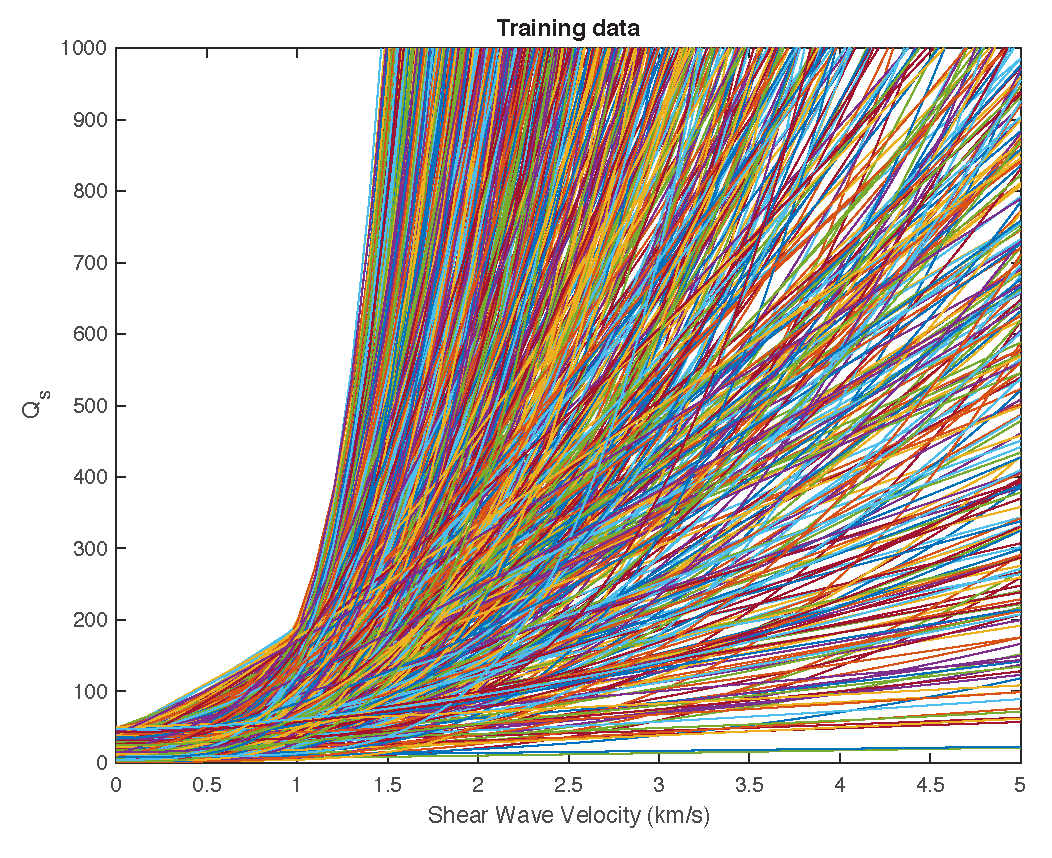
\includegraphics[width=0.5\textwidth]{figures/pdf/Figure_training_data.pdf}
    \caption{Training data is generated based on 1000 random combination of $C$, $\alpha$, and $\beta$. For statistical distribution of the input parameters refer to Fig.~\ref{fig:Figure_training_data_statistics}}
    \label{fig:Figure_training_data}
\end{figure}

 \begin{figure}[ht]
    \centering
    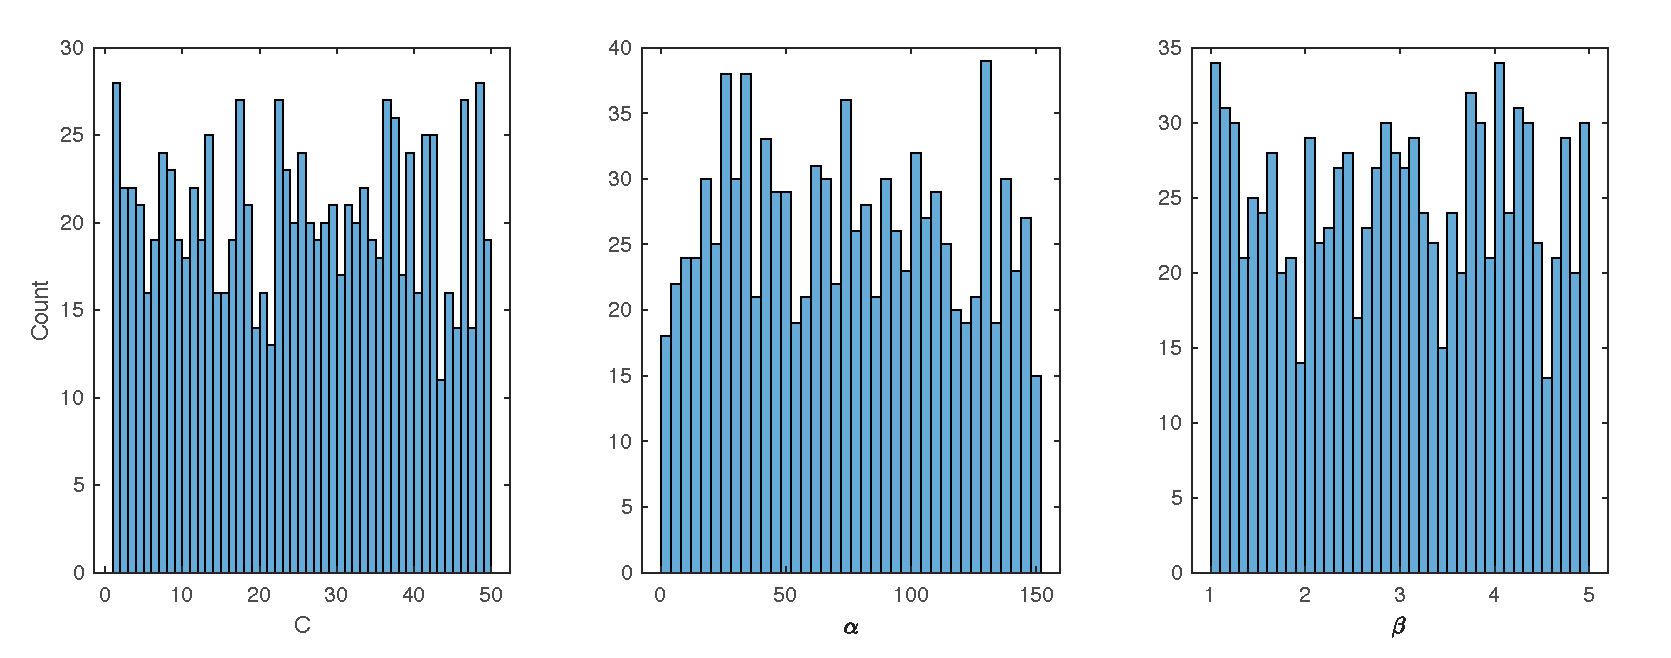
\includegraphics[width=\textwidth]{figures/pdf/Figure_training_data_statistics.pdf}
    \caption{Distribution of training data for three input parameters.}
    \label{fig:Figure_training_data_statistics}
\end{figure}

The forward problem is a nonlinear function regression using the neural network. Therefore,  a simple multi layer feedforward (wherein connections between the units do not form a cycle) perceptron should be able to train for predicting the target value. We develop two structures  of networks. One for predicting peak ground velocity (PGV) and the other for predicting PGV, PGA, SA, and area under envelope. After several try and error on the network structure we use [9,9,3] and [9,24,8] for the first and second network, respectively. Fig.~\ref{fig:Figure_ann_structure} shows the network structure. 

 \begin{figure}
    \centering
    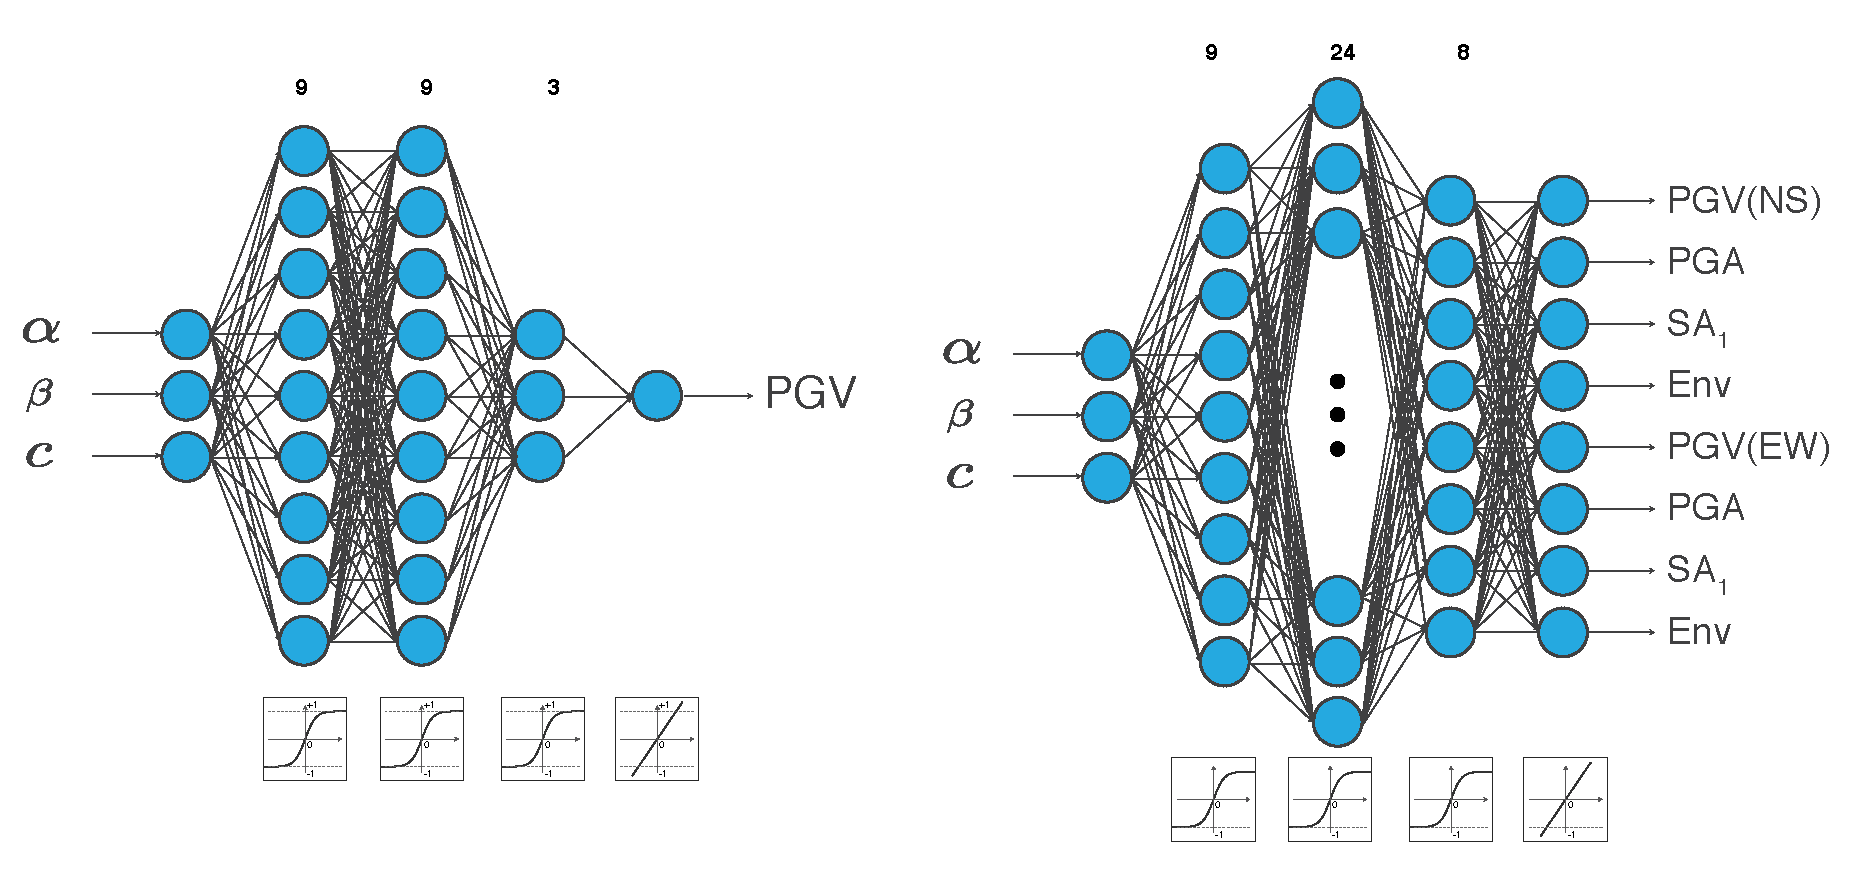
\includegraphics[width=1\textwidth]{figures/pdf/Figure_ann_structure.pdf}
    \caption{Feedforward multilayer perceptron neural networks used in the study. Hidden layers use tangent sigmoid and output layer uses linear activation functions. Dots used to simplify the structure for presenting purposes.}
    \label{fig:Figure_ann_structure}
\end{figure}

Networks have good performance during the training session. Fig.~\ref{fig:Figure_training_performance} represents the training performance for one of the networks (predict PGV). We used 60, 20, and 20\% of data for training, validation, and test dataset, respectively.  As one can see the validation data set stops training process when it is prone to overfitting as we can see the training RMS is decreasing significantly. 

  \begin{figure}[ht]
    \centering
    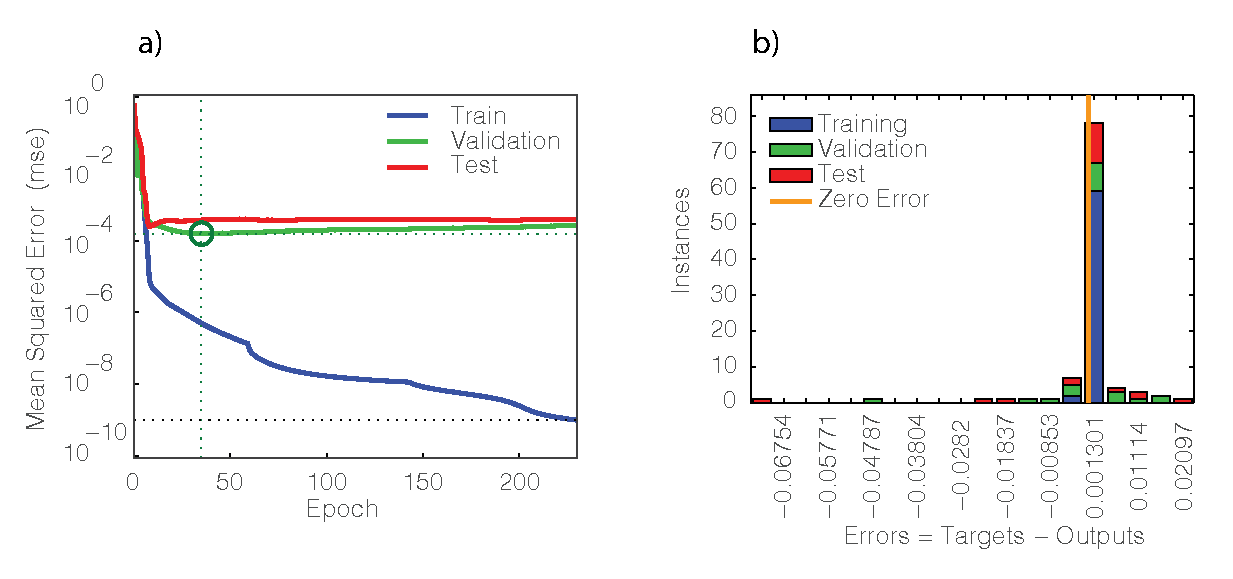
\includegraphics[width=\textwidth]{figures/pdf/Figure_training_performance.pdf}
    \caption{a) Train, Validation, and Test performance. b) Error histogram}
    \label{fig:Figure_training_performance}
\end{figure}

Although we report each trained network functionality and review them after training and optimization process, we do not review each individual of them before using in the optimization process. Therefore, in order to increase the network generalizability and performance we use ensembling method through bagging approach. First we hold 5\% of data out of dataset for final test and use  85,15 \% of remaining data into training and validation. Then we generate 10 different neural networks. Defining 10 different networks help to decrease the chance of overfitting and in the most of the time provides very accurate results.  Since assigning training, validation, and test dataset is randomly done, these networks are trained based on different data. Our results show that ensembling method significantly improve the results. Fig.~\ref{fig:Figure_ANN_num_training_data_sens}.a shows that increasing number of training data, in general, reduce the RMS error for test data. Fig.~\ref{fig:Figure_ANN_num_training_data_sens}.b represents accuracy of training network with 100, 400, and 1000 training data on test dataset. As we can see in the case with 100 training data, each individual network is far from the actual value, however, ensembling method average them out and brings them close to the actual value. 

  \begin{figure}[ht]
    \centering
    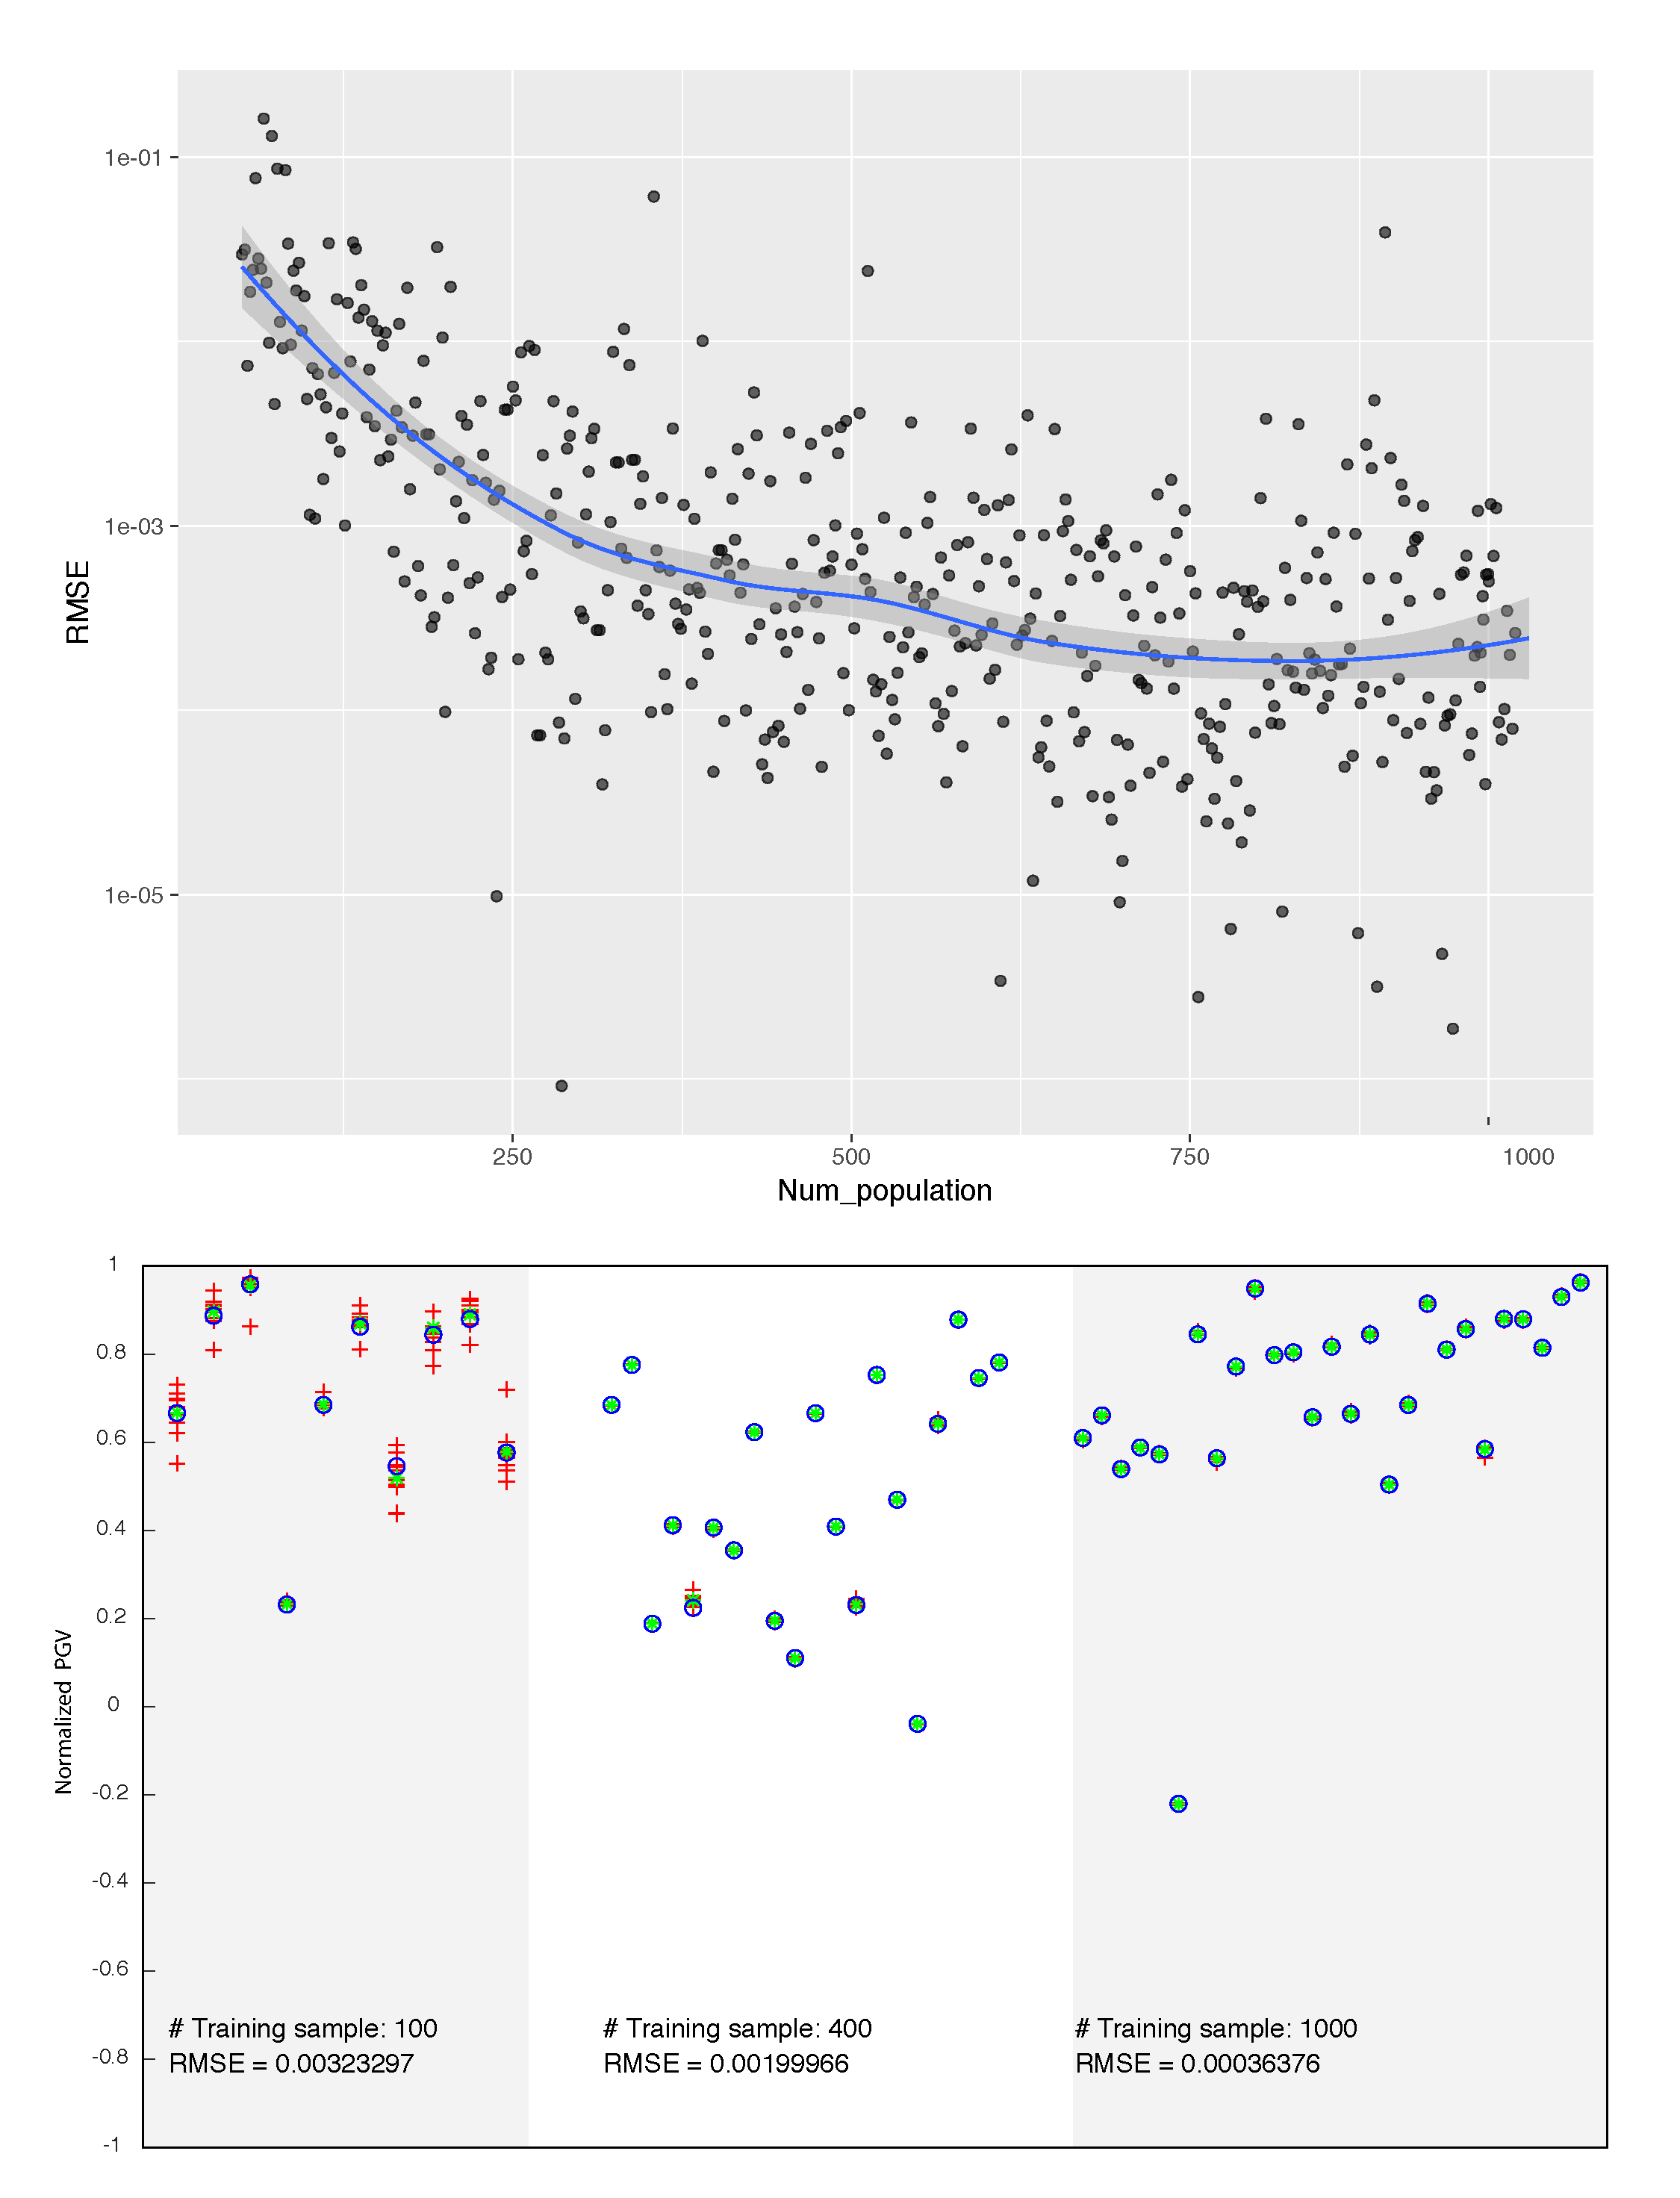
\includegraphics[width=0.7\textwidth]{figures/pdf/Figure_ANN_num_training_data_sens.pdf}
    \caption{Variation of RMS error with increasing number if training data and examples of predicting target value in actual simulation}
    \label{fig:Figure_ANN_num_training_data_sens}
\end{figure}


%The objective of this study is to propose a method to accurately search for the best parameters for anelastic damping. The idea of comparison of data and simulation is not a novel thing, however, traditional methods, which is using direct forward simulation, can cost significant computational resources and time. Therefore, we show that an artificial neural network can be used to accurately estimate the target parameter (in this case geometric mean of peak ground velocity).  And with it's combination with optimization process and conducting study on the same domain, however, predefined damping parameters, one can estimate the effective shear wave velocity of the results of that station and focus on those results in comparing with actual observation. Also we show that for each station An optimization process needs to evaluate the proposed parameters numerous time, if we consider only one time evaluation for each time-frequency window of each station, we will need 13100 $(262(stations)*10(time-window)*5(frequency-band))$. Whereas we know an optimization process evaluates the hundreds of thousands times. In this study we show that we can get the same results with significantly lower number of regional scale simulations (220 simulations). 

%In this section we first study the variation of peak ground velocity with different parameters. Then we provide an overview of the trained network and their overall accuracy. We continue with a review of optimization process and we provide a couple of examples of the results. We study different combinations and how results can be different. We also show that how ANN is unable to learn a good network based on noise-windows. After comprehending different types of results, we present the variation of parameters regarding the time windows, frequency bands and stations distance.  

%Modifying anelastic attenuation parameters has considerable effects on the final results. Fig.~\ref{fig:Figure_6_q_models_hypo} shows different plots based different parameters.

% \begin{figure}
%    \centering
%    \includegraphics[width=\textwidth]{figures/pdf/Figure_6_q_models_hypo.pdf}
%    \caption{Processing steps}
%    \label{fig:Figure_6_q_models_hypo}
%\end{figure}

%As one can see variation of these parameters change the overall trend, however, it is not an easy task to find the best parameters without a well defined optimization system. This becomes complicated when we discuss about different frequency bands as well. Therefore, We generated sudo-simulator to do numerous large number of simulation without actual simulation using neural networks. As we discussed in the methodology section, we generated 1000 training data. The generated training data are shown in Fig.~\ref{fig:Figure_training_data}.



%However, our analysis show that, defining higher c values (more than 50) extremely reduce the functionality of the network. The reason for this happening is higher Q values give almost the same results therefore it becomes independent of the input values. Besides we believe higher c values (more than 50) is not practical (in a relationship which already has other terms which increase Q values with respect to shear wave velocity). Therefore, we reduce the training data into 215 data that includes all values with c less than 20. All previous studies show that Q factor increases with increasing shear wave velocity therefore we considered beta to be in the the rang of $[1,5]$. previous studies suggest that alpha should be around $50-100$ we set our searching domain in $[0,150]$. Therefore, each time-frequency window of data has 1000 training data. The generated training data are shown in Fig.~\ref{fig:Figure_training_data}.b represent the set of data that is used for training process. Fig.~\ref{fig:Figure_training_data_statistics} show the distribution of these data.  



  %After several try and error we choose a structure with three hidden layers (9,9,3). 


The generated networks are fed into optimization process where the optimization cost function use the combination of these networks as well as the value of the observation (either synthetic target or actual data) to find the best set of parameters for each station.  A different combination of $C$, $\alpha$, and $\beta$ can produce a very similar $Q$ value. Therefore, the optimization process does not have a global minimum, rather many local minimum which are fairly close together, (although one set of parameters can ends up to the least value and become a global minimum, that slight differences is not what we are interested in this study.) In result, we go through the optimization process from different initial point, which are randomly set, to have several optimum parameters. We repeat this process 50 times and report the results. Generating numerous optimum values for each station helps to understand at which velocity range the solution converges. We study this by mean and standard deviation of the results. In case of the checkerboard resolution idea, the optimized results should be very close if not the same in the effective/dominant shear velocity range; and we expect to see fairly different results at non-effective shear wave velocity ranges. In the following we present the test of method on idealized domains. 

\subsection{Homogeneous domain (H1)}

The first idealized domain is a homogenous domain with shear wave velocity of $1000 km/s$. For more information about domain details and stations location see Fig.\ref{fig:3d_domain_scenarios}. Fig.\ref{fig:record_section_1000} represents the record section of NS horizontal component for peak ground velocity. According to the figure a clear S-wave arrivals and peak value of them is obvious and easy to pick.

  \begin{figure}[ht]
    \centering
    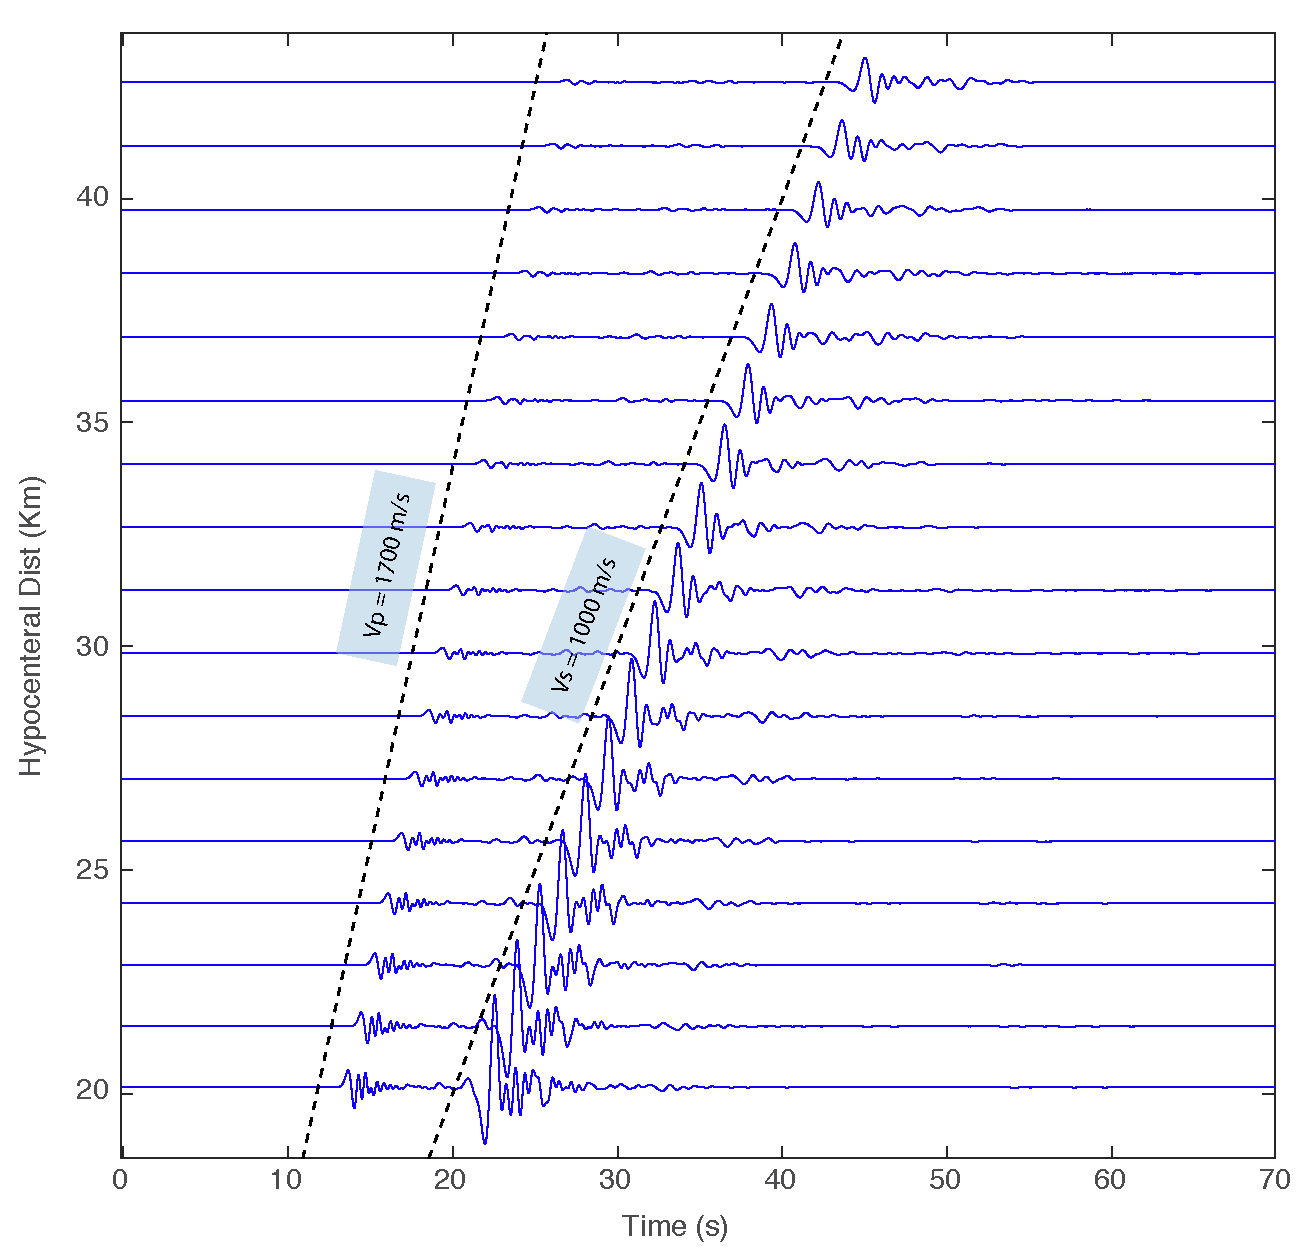
\includegraphics[width=0.8\textwidth]{figures/pdf/record_section_1000.pdf}
    \caption{Record section of NS component (H1)}
    \label{fig:record_section_1000}
\end{figure}

 We generate a test data and set the program to search for the initial parameters using stations results. Figure.~\ref{fig:station_1_1000_H1} shows the results after optimization process. We expect to see at each station, for the effective shear wave velocity (here $Vs=1000 m/s$), the optimized parameters and the target parameters Q are very close to each other if not the same. 

  \begin{figure}[ht]
    \centering
    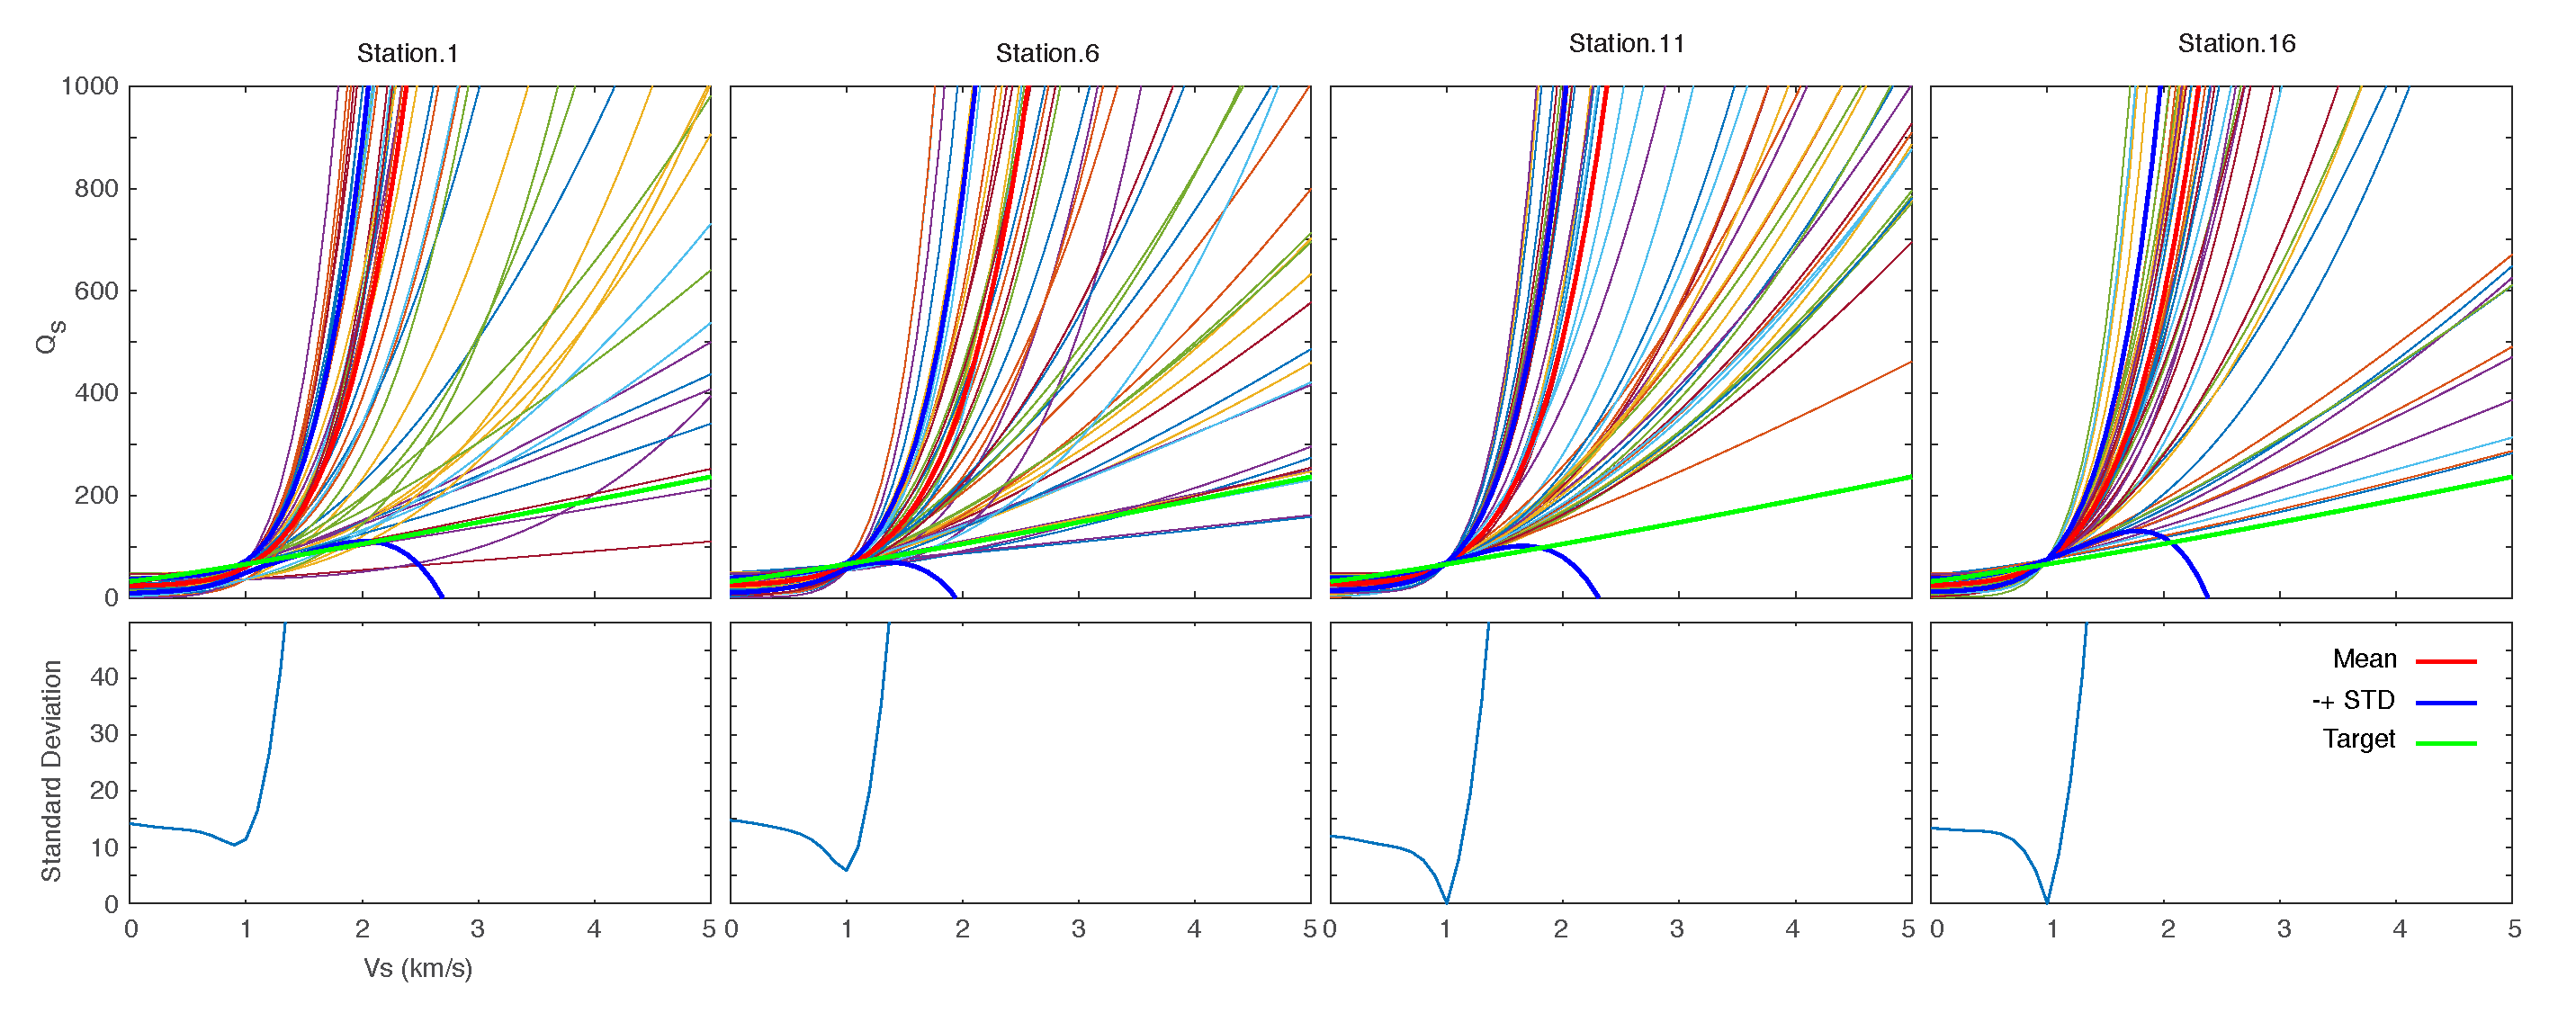
\includegraphics[width=\textwidth]{figures/pdf/station_1_1000_H1.pdf}
    \caption{Results of 50 optimized solutions for homogeneous (H1) domain for 4 stations.}
    \label{fig:station_1_1000_H1}
\end{figure}

According to the figure which is results of several stations, we can see not all stations are accurate in picking up the results, specifically, closer stations are not good detectors. That is understandable, because at the closer stations the wave does not have chance to travel enough to capture the anelastic damping characteristics. On the other side, far stations have almost zero standard deviation meaning that all individual results have the same value at the effective shear wave velocity. This test gives the idea that for simple case if we can accurately pick the peak ground velocity, at considerable distance from the source, our optimization process can accurately estimate the Q value for dominant/effective shear wave velocity. Also it empower the idea that we should not treat all stations the same. The closer stations are not as accurate as farther stations in picking up the input parameters. 

\subsection{Layered domain (L1)}

We add a shallow low velocity zone to the H1 domain. Figure.~\ref{fig:station_1_1000_500_L1} shows the results after optimization process. According to the results, as we observed in the homogeneous domain, closer stations to the source are not so accurate, with increasing distance standard deviation decreases and also in mid-distance we can see effective shear wave velocity is in the range of $0.8-1 ~ km/s$ whereas at the  farthest station with respect to the source the effective shear wave velocity is $1~km/s$. This is another indication of successful detection of dominant/effective shear wave velocity in a layered domain.  

  \begin{figure}[ht]
    \centering
    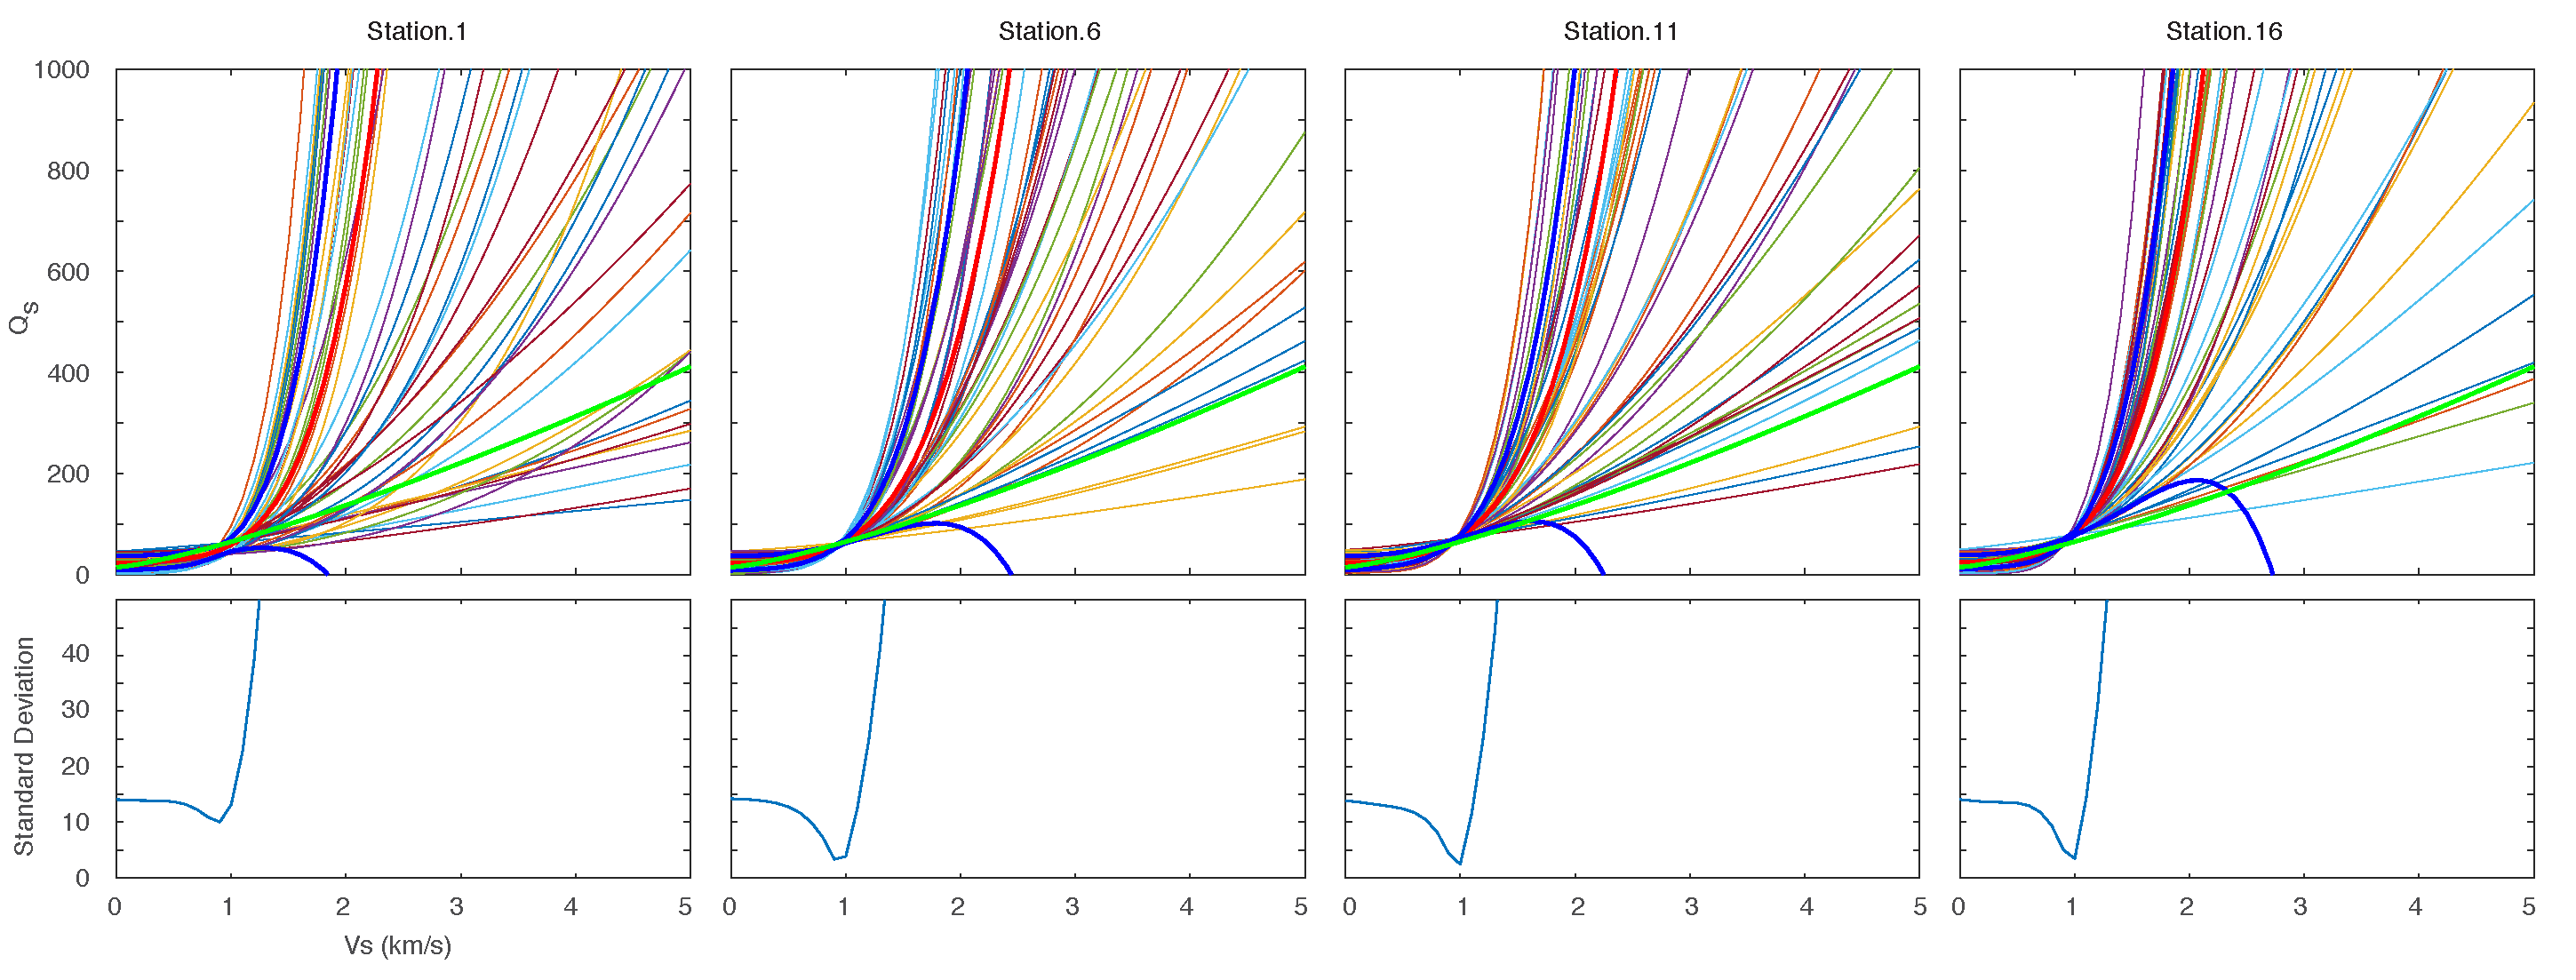
\includegraphics[width=\textwidth]{figures/pdf/station_1_1000_500_L1.pdf}
    \caption{Results of 50 optimized solutions for Layered (L1) domain for 4 stations.}
    \label{fig:station_1_1000_500_L1}
\end{figure}

It is worth mentioning that effective/dominant shear wave velocity that is detected in this idealized scenario is not used in the simulation domain. However, the value is according to the input parameters. What is important is detecting accurate Q value for appropriate shear wave velocity. 


\subsection{Layered domain (L2)}

We increase the depth of low velocity zone of L1 domain (from 256 to 1024 m) to see if the effective shear wave velocity of each stations has a considerable changes. Figure.~\ref{fig:station_1_1000_500_2_L2} shows the results after optimization process. The results show that the effective shear wave velocity becomes a little less than $1~km/s$. It is understandable; because in this scenario the $500~m/s$ low velocity zone can have more effects on propagated waves.  The idea of effective shear wave velocity or average shear wave velocity is not a novel concept. It is used in many different application to estimate the overall shear wave velocity of a soil profile (e.g., see time average method for shear wave velocity in geotechnical engineering applications).  

  \begin{figure}[ht]
    \centering
    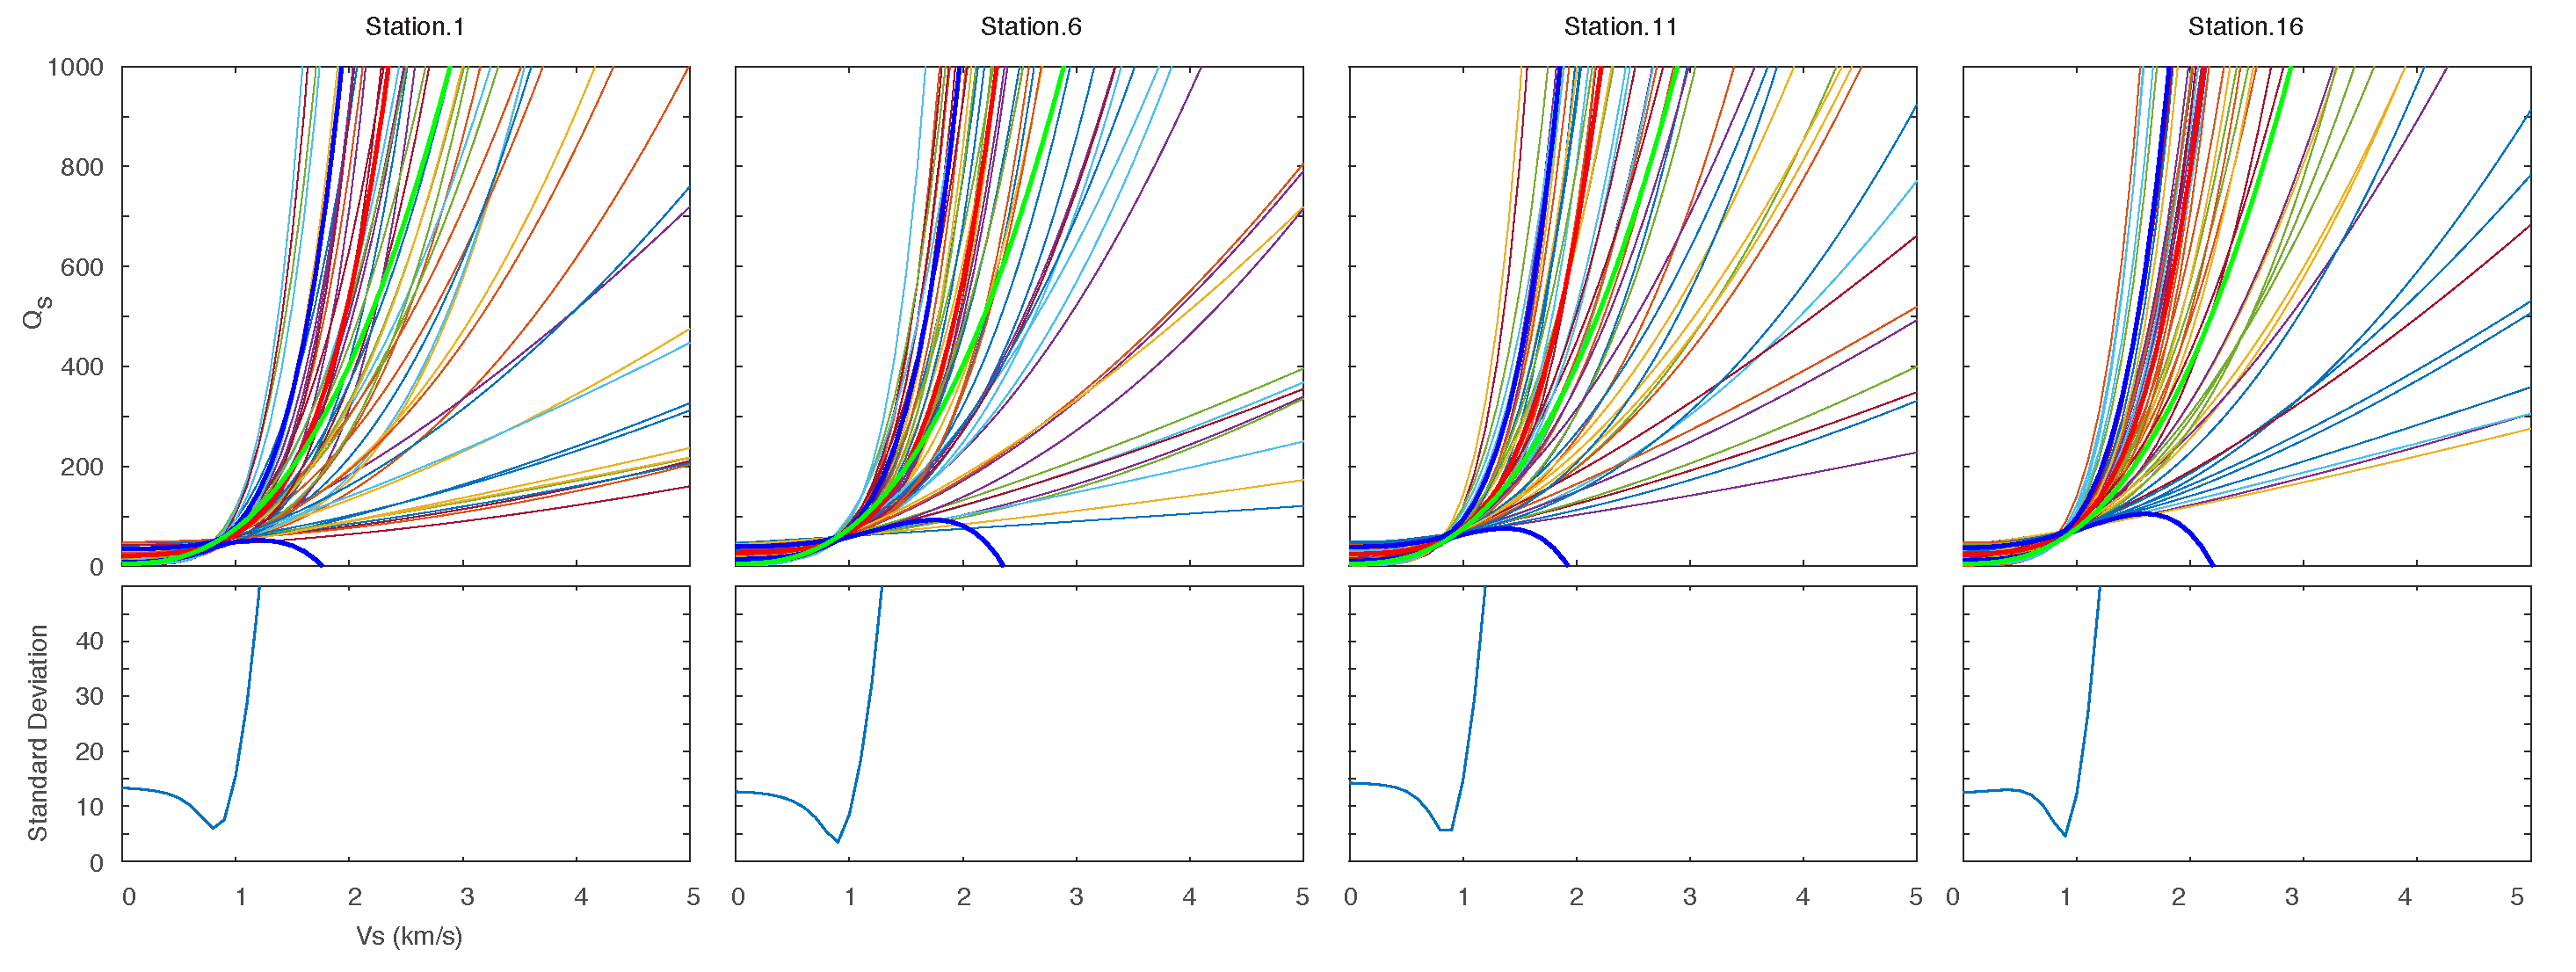
\includegraphics[width=\textwidth]{figures/pdf/station_1_1000_500_2_L2.pdf}
    \caption{Results of 50 optimized solutions for Layered (L2) domain for 4 stations.}
    \label{fig:station_1_1000_500_2_L2}
\end{figure}

\subsection{Layered domain (L3)}

We tried another idealized layered profile with three different layers. According to Fig.~\ref{fig:station_1_2000_1000_500_L3_nt}, the variation of effective shear wave velocity is obvious that shifts from low velocity to higher velocities with increasing the distance from source. 

  \begin{figure}[ht]
    \centering
    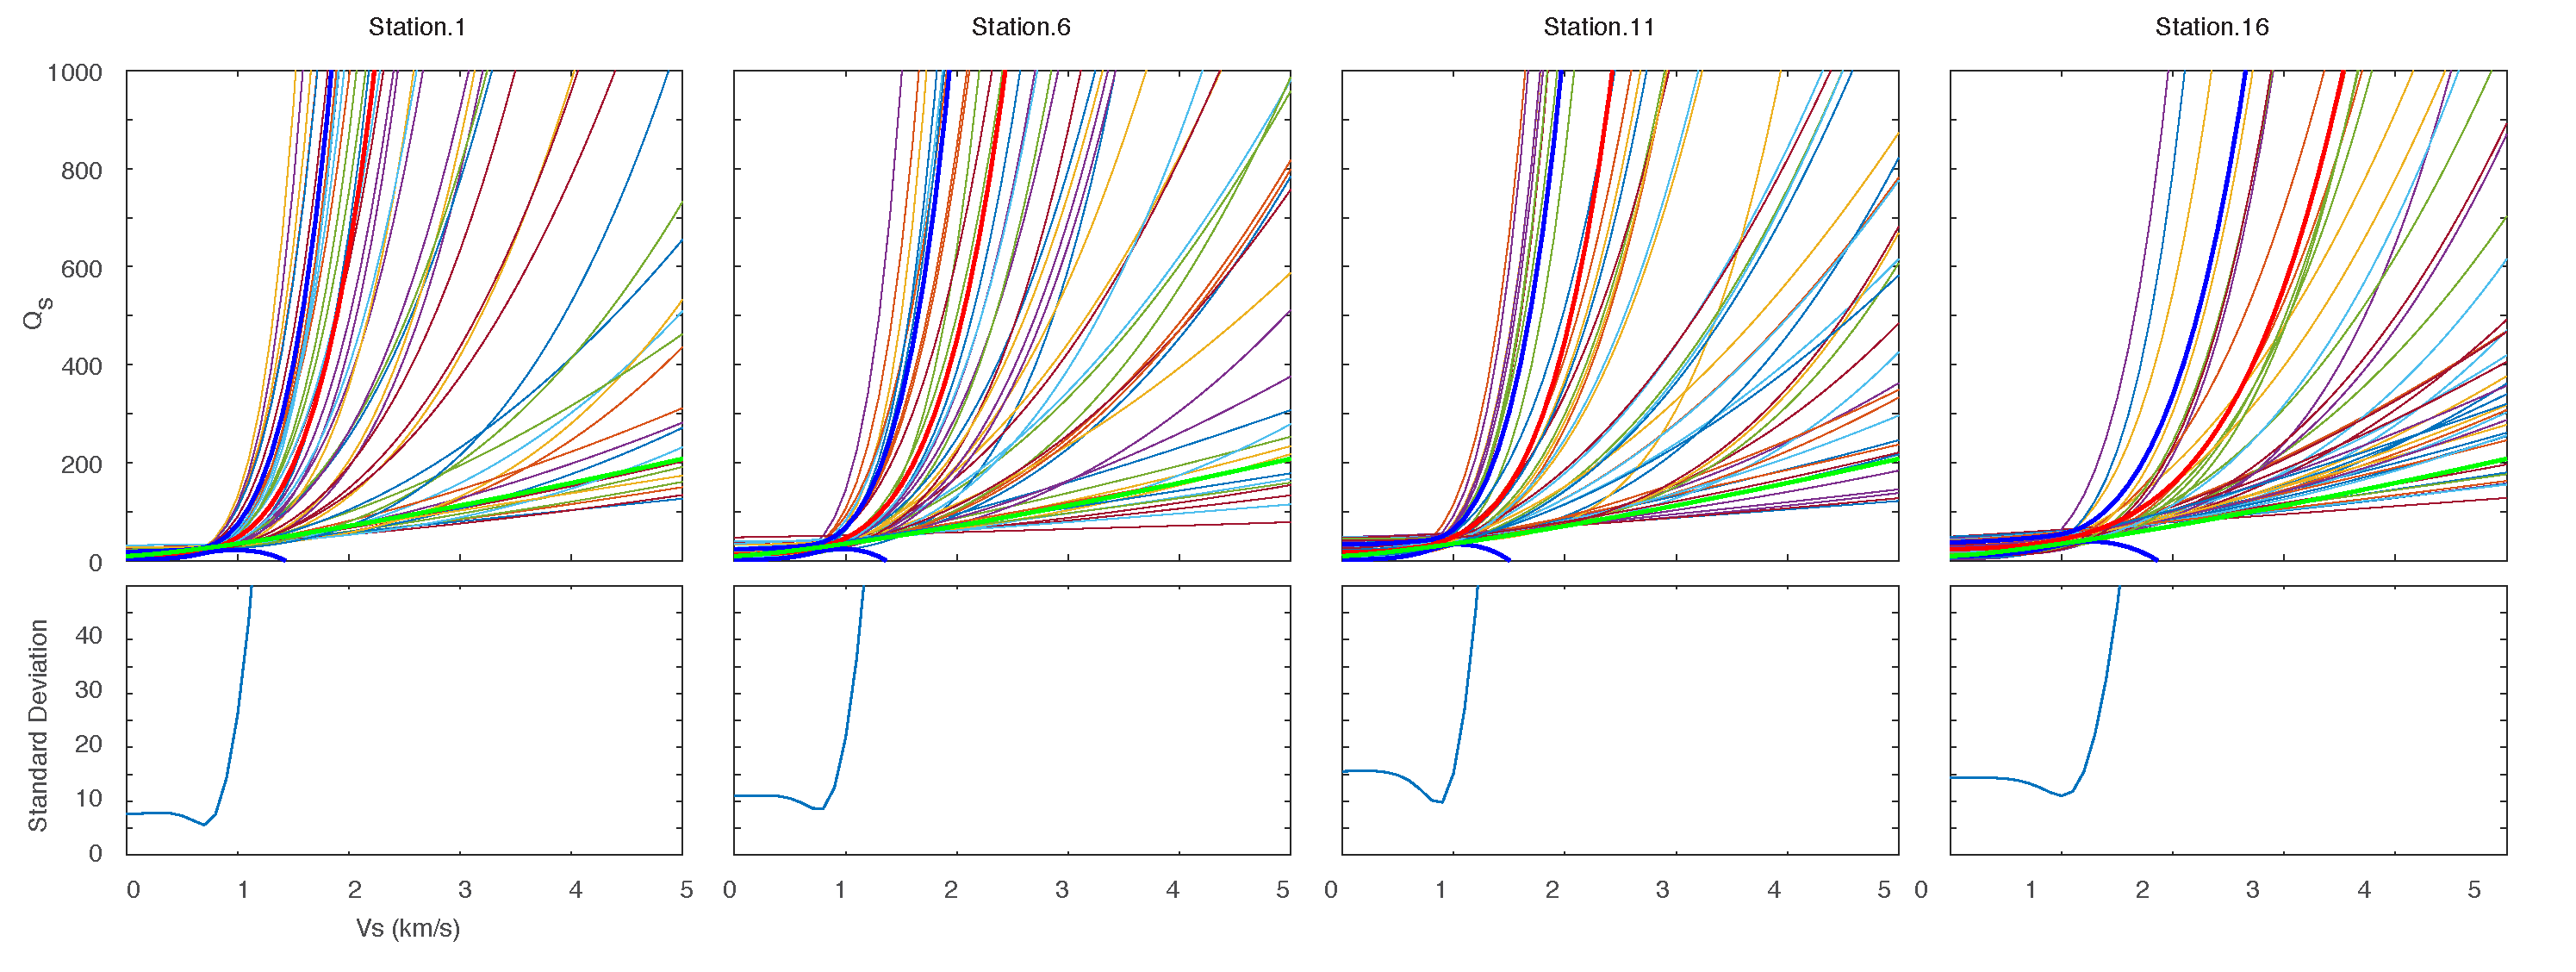
\includegraphics[width=\textwidth]{figures/pdf/station_1_2000_1000_500_L3_nt.pdf}
    \caption{Results of 50 optimized solutions for Layered (L3) domain for 4 stations.}
    \label{fig:station_1_2000_1000_500_L3_nt}
\end{figure}

However, we do not see a good convergence rate. The standard deviation of the optimum results around the effective/dominant shear wave velocity is slightly lower, but it is not as sharp as simple domains (e.g., H1). We achieved similar results for heterogeneous domain, as well. With increasing domain complexities, determination of effective shear wave velocity is not as sharp as before. It suggests the idea that peak ground velocity may not be enough to estimate the results. Please note that the idealized scenario does not have a common ambient noise that the normal observational data have. Therefore, we can say peak ground velocity is not enough and we need to add more parameters to better estimate the results. In the next section we study other metrics possibility in determining the results. 

\subsection{Alternative metrics}

Neural networks proved to be very good estimators for nonlinear functions. Broaden output results can help the networks to learn accurately. With broaden we mean more variable output results. However, non-broaden target results, have a behavior very similar to noise and make the training process very difficult. In other words, the network estimate a parameter which is not accurate. In terms of estimating the parameters for Q factor, in complicated domains due to different wave reflections and refractions from complicated geology, peak ground velocity becomes less sensitive to these input parameters. Therefore, in this section we study the coefficient of variation (CV) as a measure of relative variability of PGV,  PGA, Area under the signal envelop, and Response spectra. Coefficient of variation is defined as 

\begin{equation}
CV=\sigma/\mu * 100 
\end{equation}

Figure.~\ref{fig:metrics_sensitivity} shows CV for different metrics for the same training data. Higher CV indicates better possibility of training accurate neural network, which in return the optimization process can estimate accurate optimal parameters. 

  \begin{figure}[ht]
    \centering
    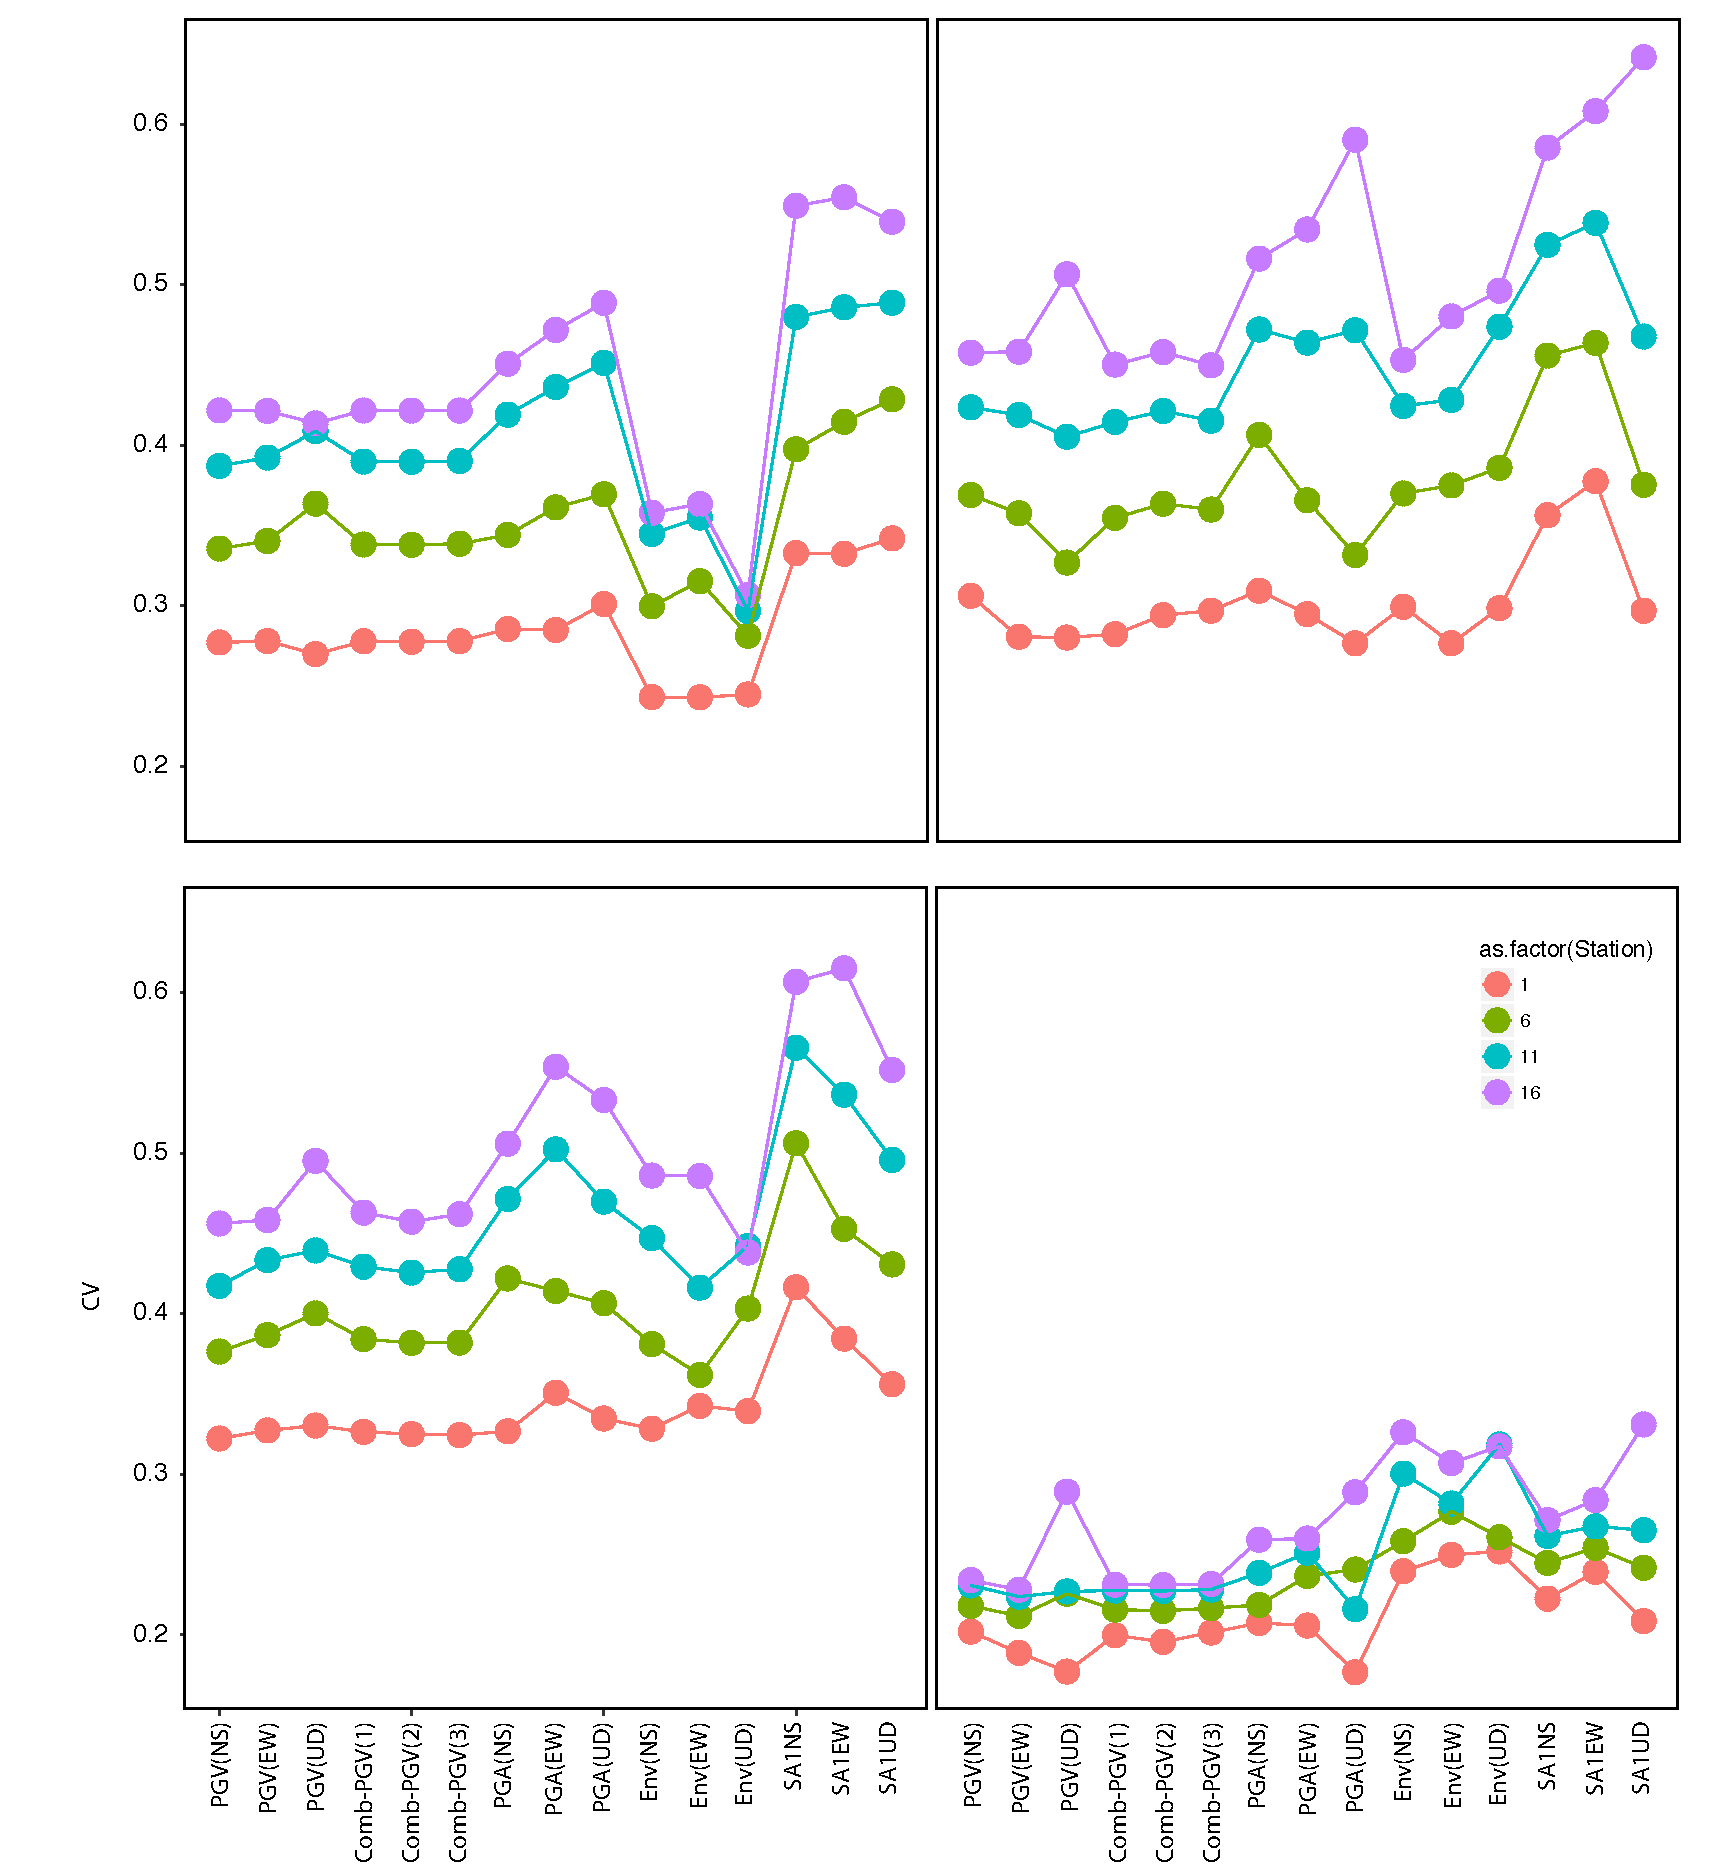
\includegraphics[width=0.8\textwidth]{figures/pdf/metrics_sensitivity.pdf}
    \caption{Coefficient of Variation of different metrics for 1000 training data.  }
    \label{fig:metrics_sensitivity}
\end{figure}

Several points are worth mentioning from Figure.~\ref{fig:metrics_sensitivity}. In all domains, CV increases with increasing distance from source. It suggests the idea that farther stations can be trained more accurately and they are much more sensitive to the variation of input parameters. Please not that all stations use the same input parameters. Previous figures show that we can optimize the results even at closer stations. However, in previous figures we represent that farther stations provide more accurate results. In the simple cases (H1,L1, and L2) response spectra at 1 second (SA1) is more variable, whereas in complicated case (L3) the envelop becomes important. Based on our numerous combination of outcomes, we use the second neural network structure where we have PGA, PGV, Env, and SA1 for east-west and north-south components. Figure.~\ref{fig:station_8_param_2000_1000_500} Shows the results of new metrics on the optimization results. 

  \begin{figure}[ht]
    \centering
    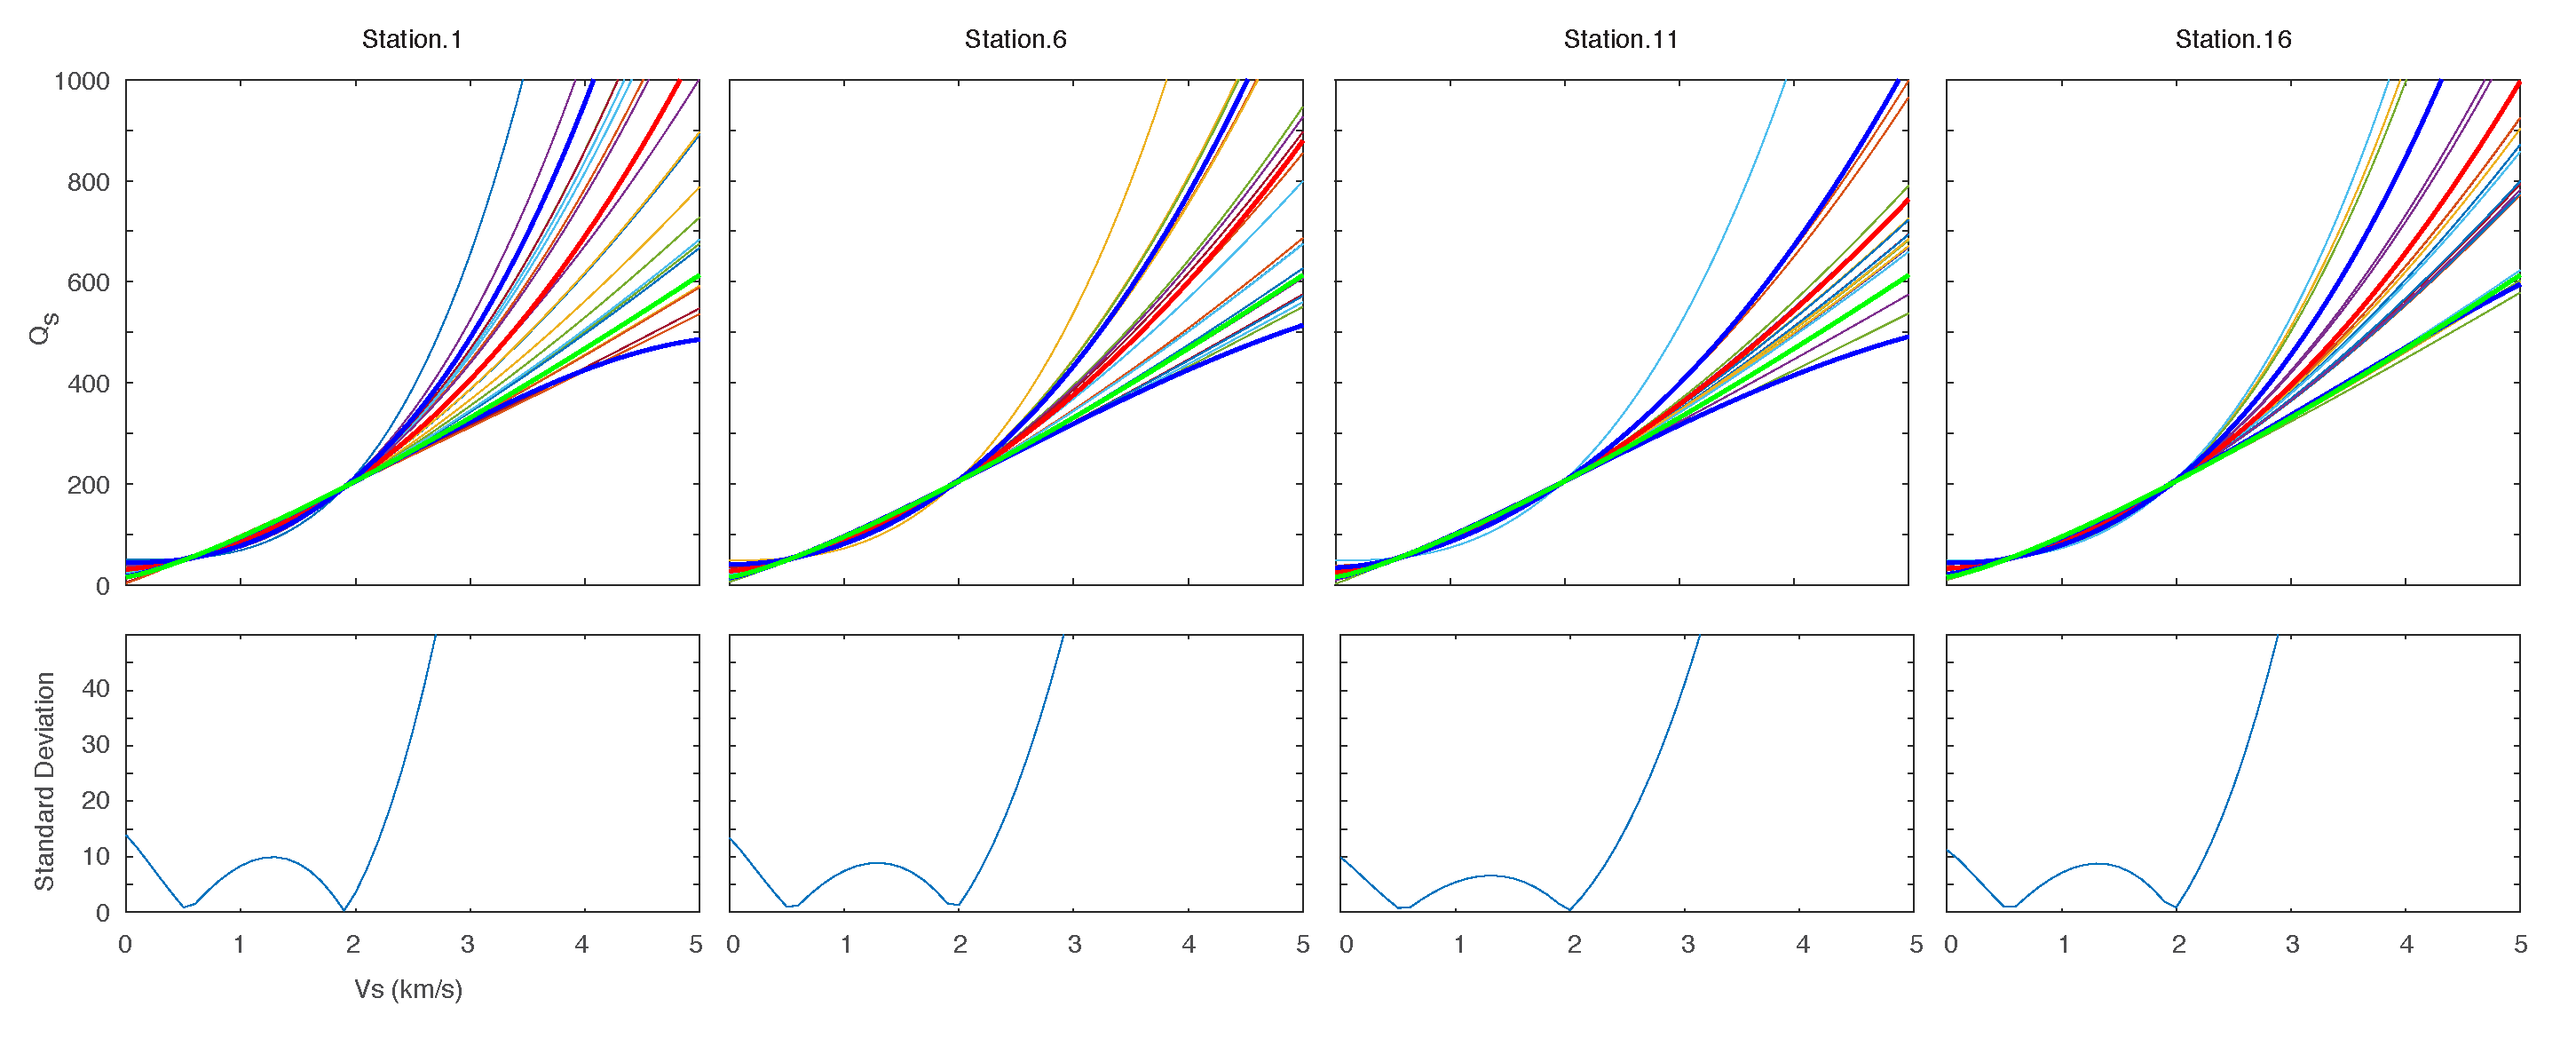
\includegraphics[width=\textwidth]{figures/pdf/station_8_param_2000_1000_500.pdf}
    \caption{SA1, PGV, PGA, Env for NS and EW component. Domain(L3).  }
    \label{fig:station_8_param_2000_1000_500}
\end{figure}

There is a significant improvement in optimization process. The algorithm can locate two of dominant shear wave velocities range which is 500 and 2000 $m/s$. The results are not accurate for 1000 $m/s$ which is not so important. Based on the metrics that are used, and the optimization process, we know that we cannot be confident about the results of 1000 $m/s$. Therefore, in the case of actual data we only use those velocity range that provide accurate results and we ignore the rest of the data.\\
Based on these results we move forward with heterogeneous domain and simulate 2008  $Mw~5.4$ Chino Hills earthquake. The simulation domain and parameters are discussed in the study region section. Figure.~\ref{fig:ANN_accuracy_stations_122_heterogenous_sim_177} shows the accuracy of the neural network for 8 output parameters for a station in the heterogenous medium. According to the figure and RMSE results, ANN can accurately be trained to estimate the requested parameters. We went through all stations, and almost all of them are similar to this stations results. Please note that the 50 test data which is used here have never been seen with algorithm during the training session. Only second test data shows slightly different results for one or some of ANNs. This also suggests the idea that 1000 training data may be is more than necessary. 

  \begin{figure}[ht]
    \centering
    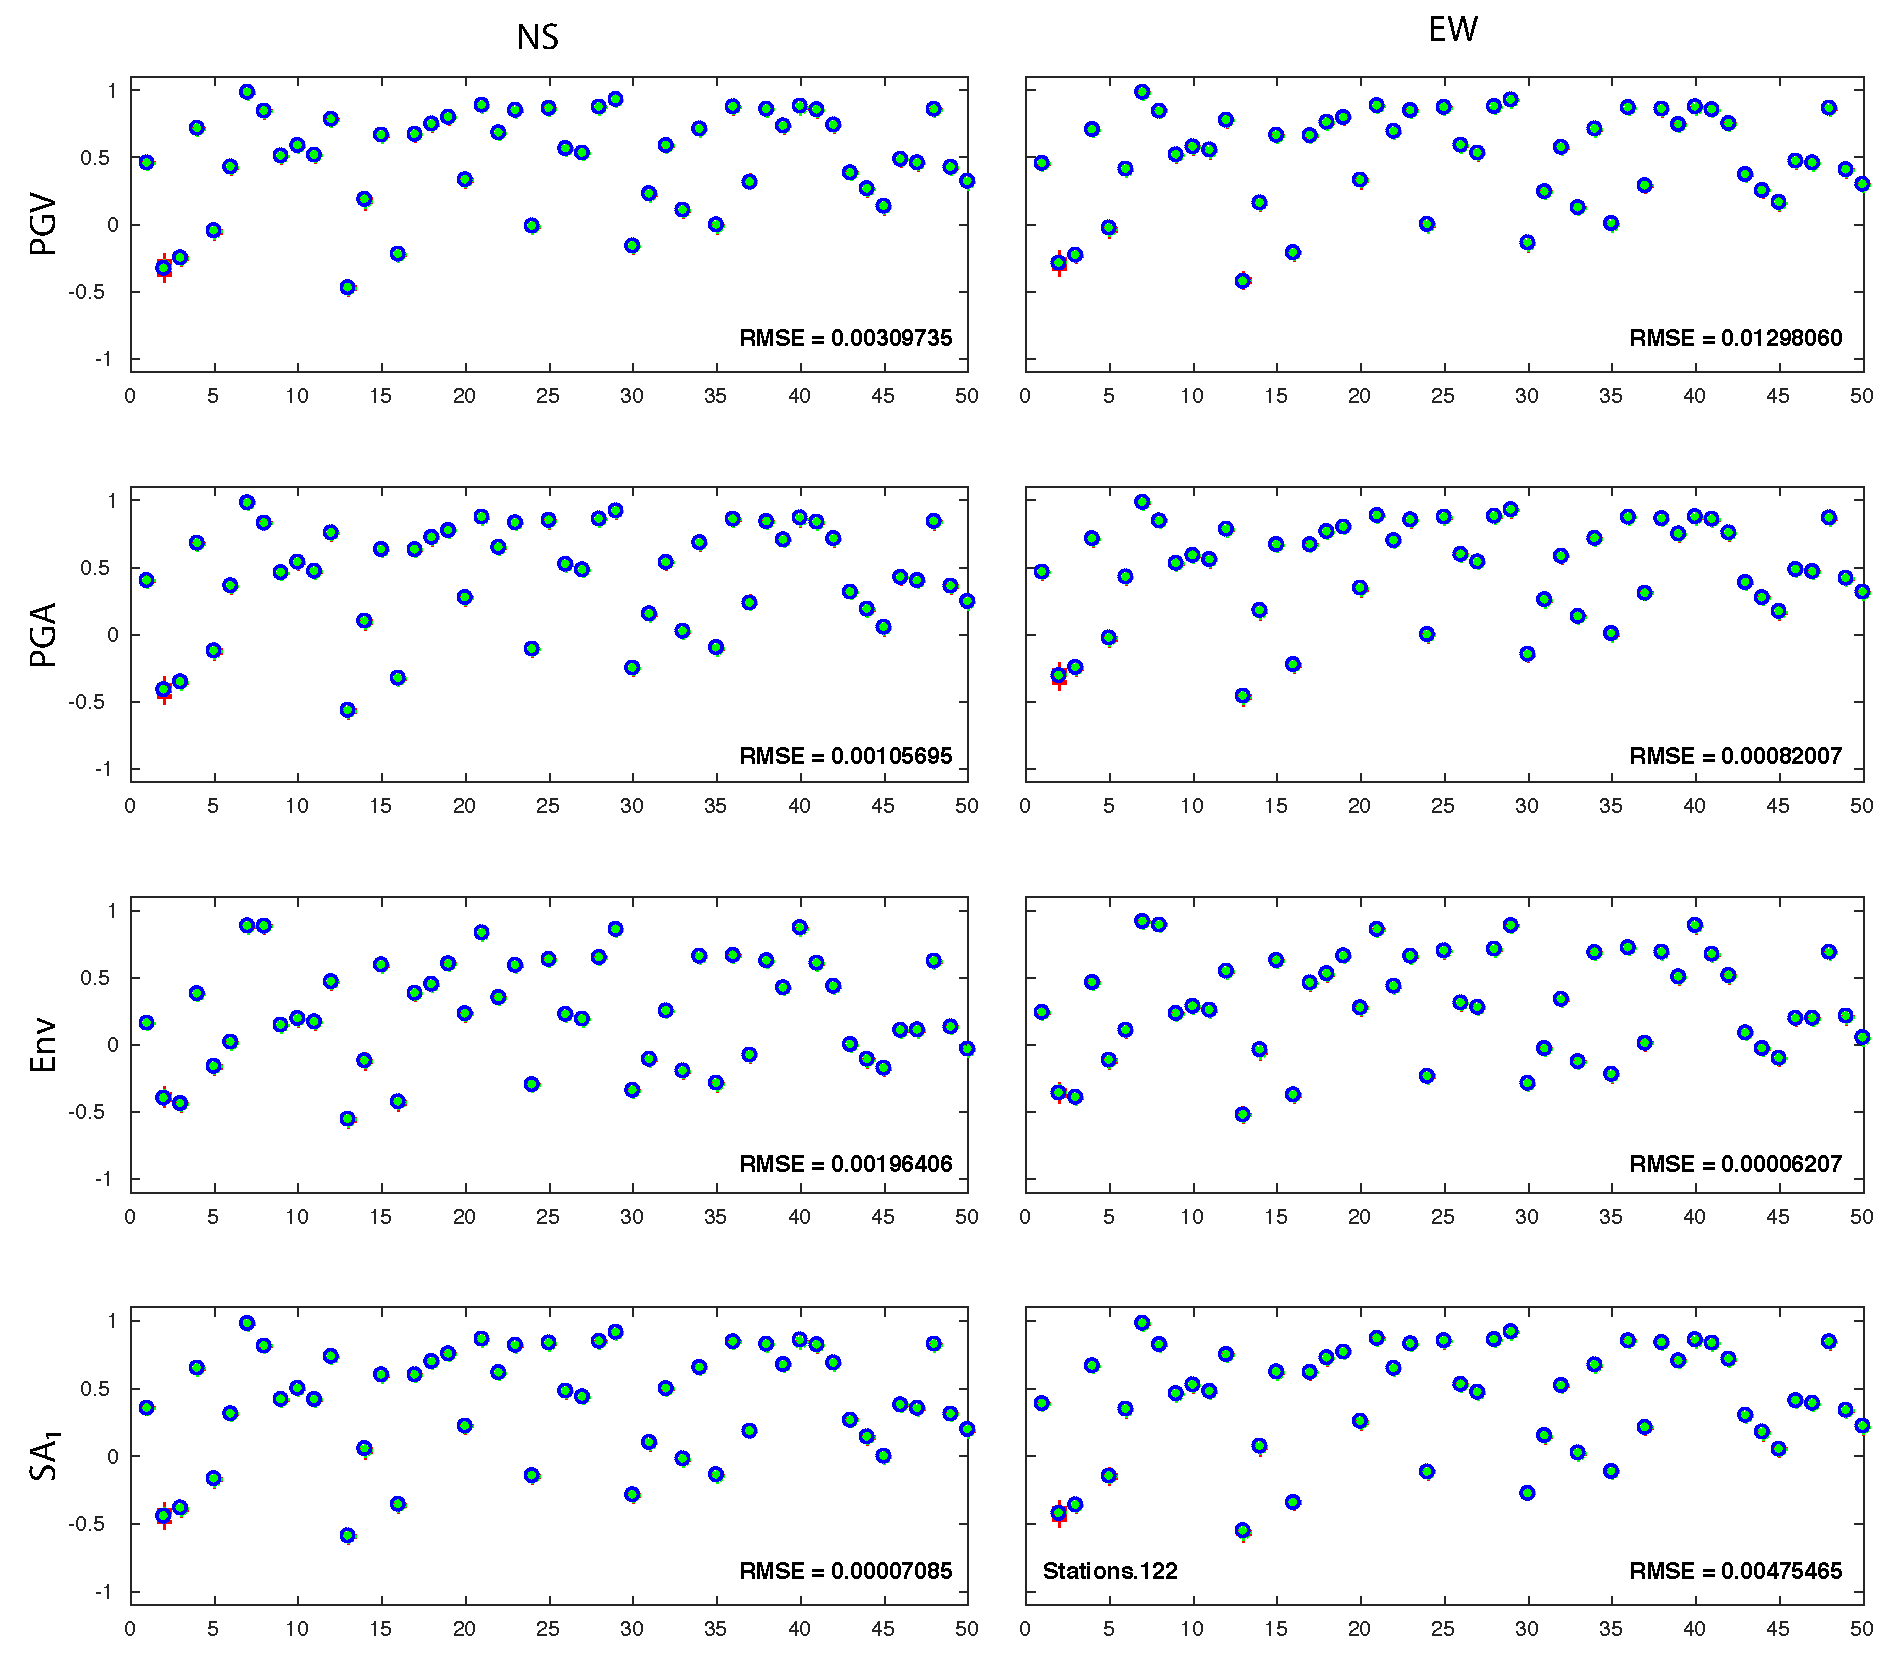
\includegraphics[width=\textwidth]{figures/pdf/ANN_accuracy_stations_122_heterogenous_sim_177.pdf}
    \caption{Accuracy of the results for station number 122 in the heterogenous domain. The station is located in about 42 km from the source (hypo central distance).  }
    \label{fig:ANN_accuracy_stations_122_heterogenous_sim_177}
\end{figure}

According to what we explained in the methodology section and idealized tests that presented here, first, we train the network for each station, then we run optimization process with considering the actual observation as a the target value. We compute the mean of 50 optimized Q values and find the closest Q equation in the training data. We run the optimization process for estimating the new test value which is very close to observation. This process helps us to understand whether the optimization process can find the actual results where we know the input parameters before hand and is very close to the potential field parameters. Those data which pass the following checklist are added to the final Qs-Vs dataset. The criteria is according below:

\begin{itemize}
\item If synthetic solution is converged for a range of shear wave velocity (Standard deviation is an indication of this situation)
\item If the optimizaiotn process successfully locate the input parameters
\end{itemize}

After passing these steps, we generate a dataset and compute another regression analysis to estimate the Qs-Vs relationship. As we can see from idealized domains, not all stations are good to extract relevant information, and not all metrics are good to extract all velocity information. This fact also happens in heterogenous domain with fairly complicated source model. Here we show four stations that some velocity range of them can pass the defined criteria. Figure.~\ref{fig:used_stations_example} shows some of these stations. 

  \begin{figure}[ht]
    \centering
    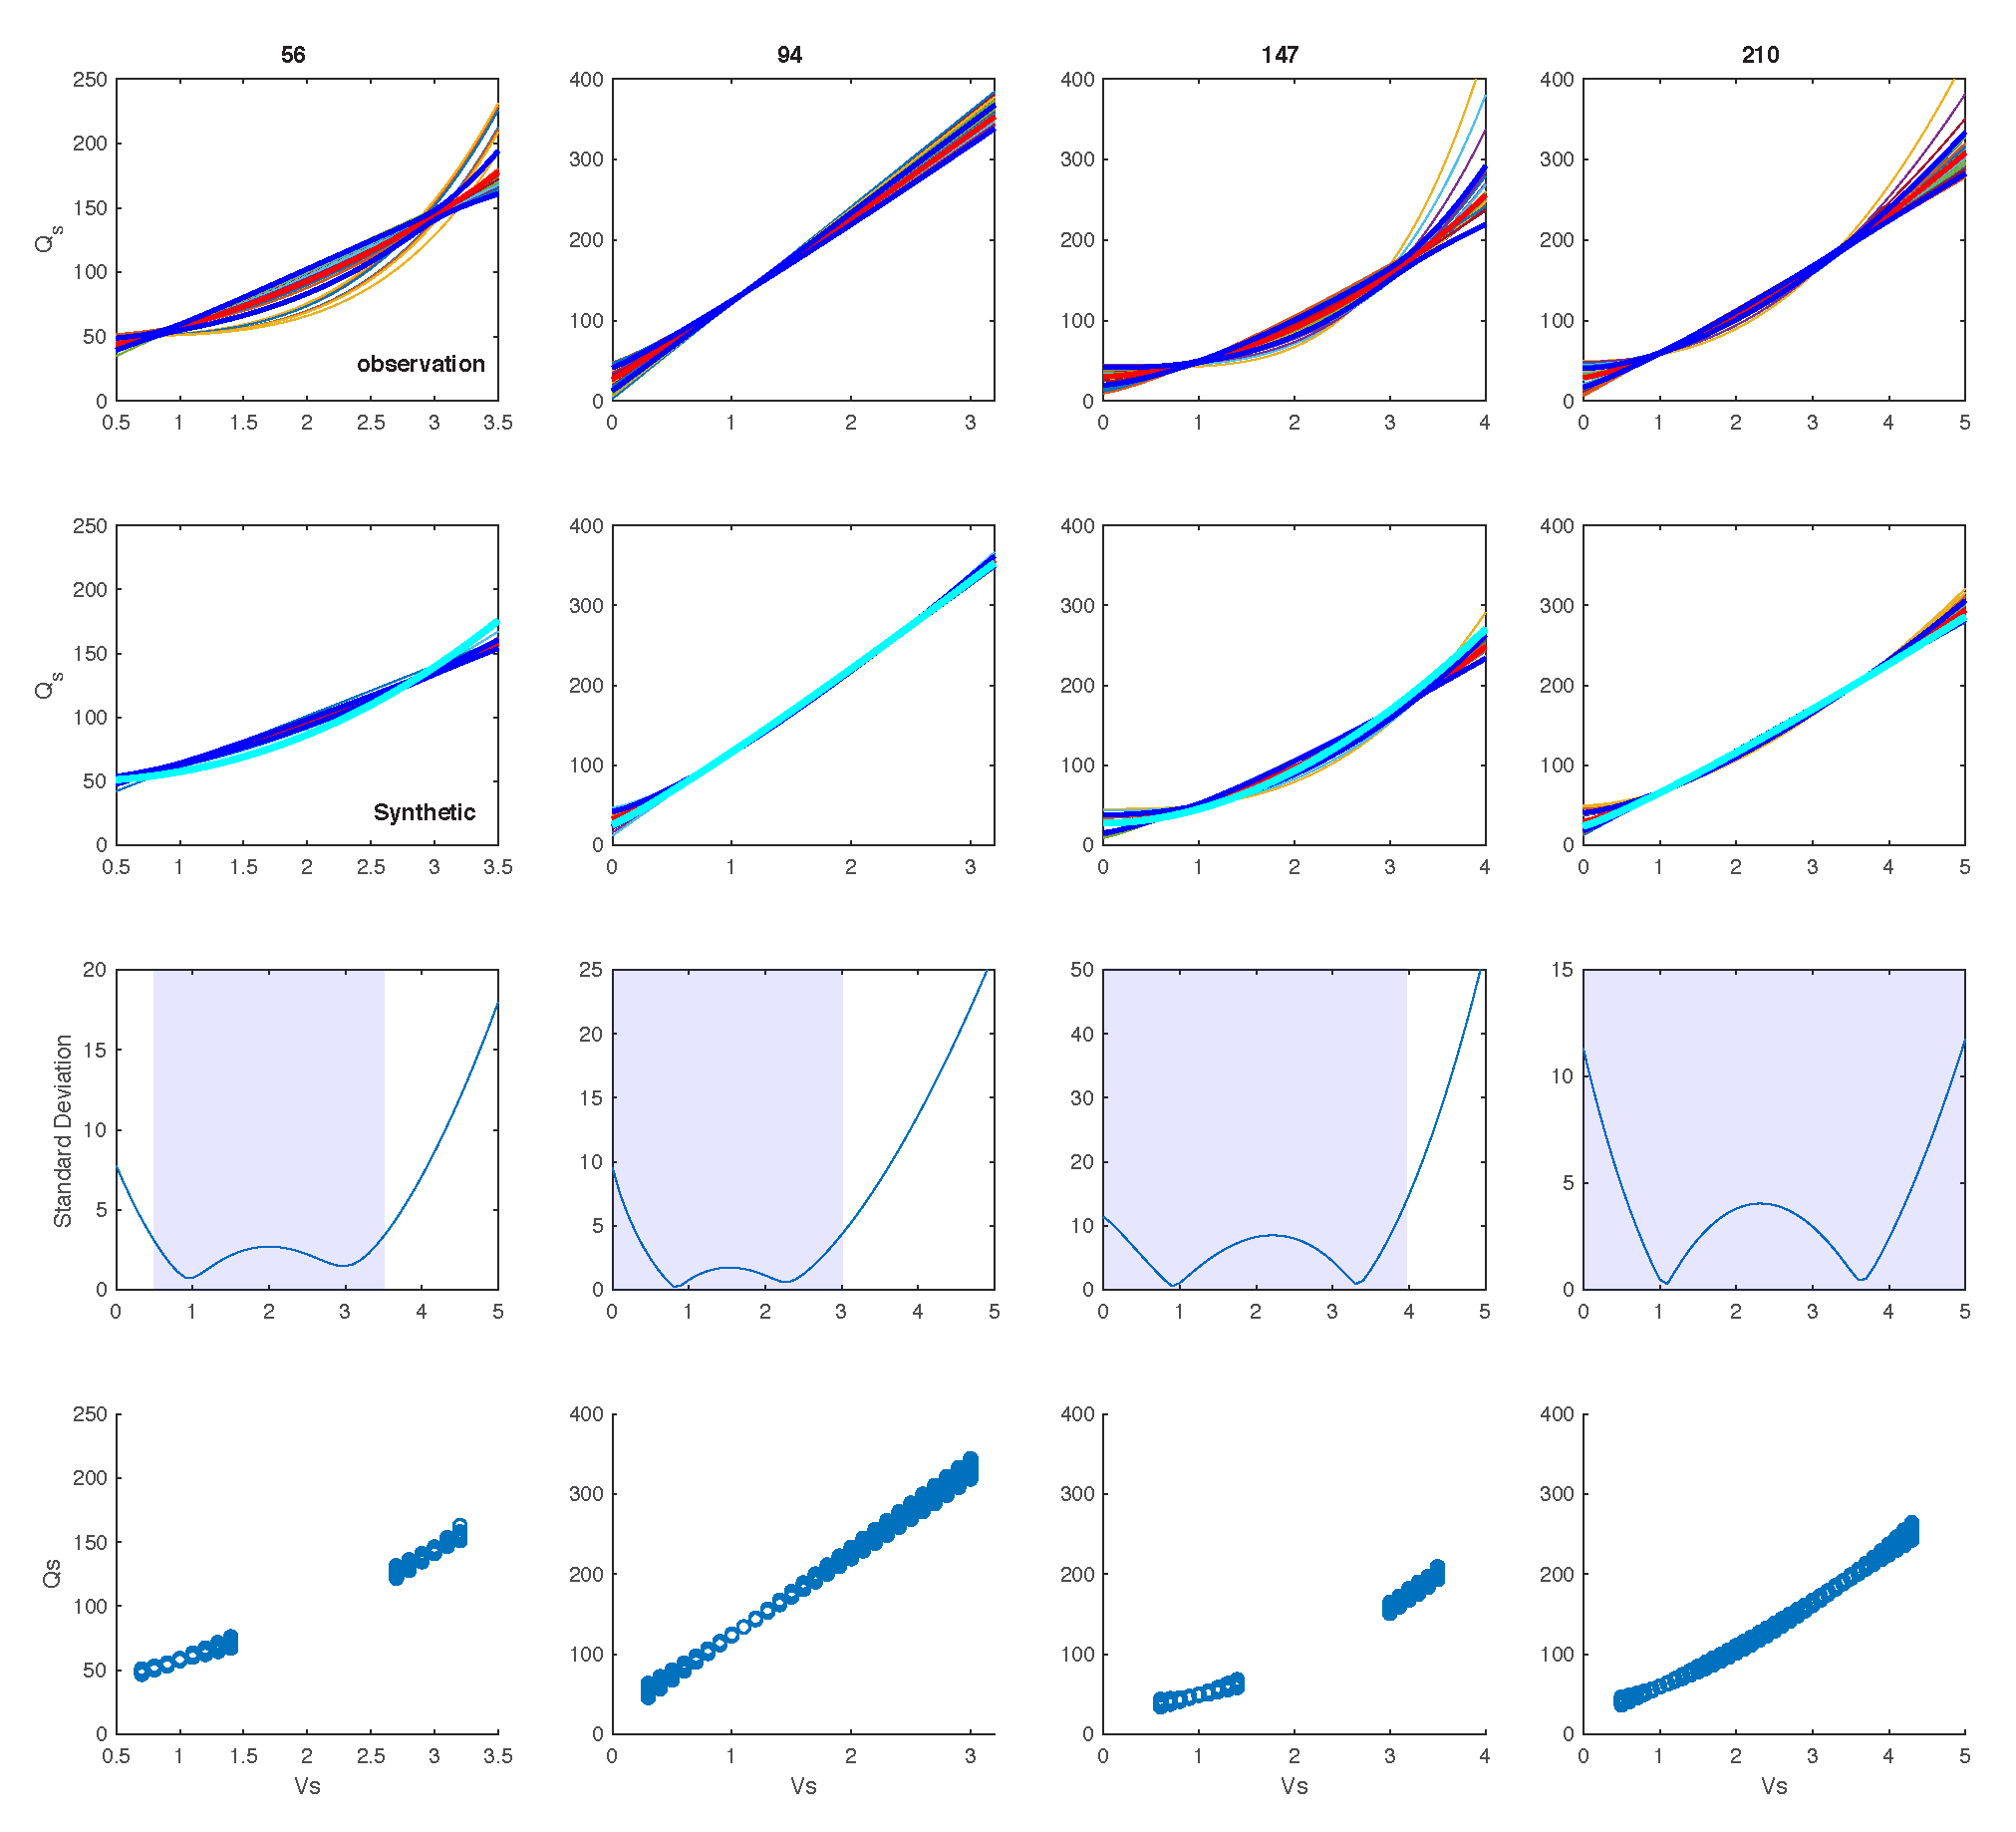
\includegraphics[width=\textwidth]{figures/pdf/used_stations_example.pdf}
    \caption{Some of stations in the heterogeneous domain that pass the criteria. The cyan line in synthetic represent the closest available data in training dataset.}
    \label{fig:used_stations_example}
\end{figure}

These four stations are example of stations that part of their shear wave velocity range are used in the final analyses. Each station provides enough information for different range of shear wave velocity. The observation and synthetic are converged at fairly close shear wave velocity ranges for both observation and synthetic. Also in those ranges the algorithm can successfully retrieve the Q value parameters that is used as an input for synthetic target value. The mentioned criteria are met and we can use the results of observation in that range. In order to choose more conservative values for each appropriate shear wave velocity we use only those data that are between $+-$standard deviation.\\
 Similar to the idealized cases, there are stations that cannot pass the defined criteria. There are several reasons worth mentioning. Some stations' results are higher than even without damping simulation. Moreover, in some stations not all metrics fall in the min and max of our training dataset. In order to involve these stations, we need to broaden our training dataset, however, estimating the accurate Q value for Los Angeles basin is not primarily task of this study. With comparing our training dataset with proposed Qs-Vs models we can say we have a very good search domain. We also should acknowledge the fact that there is a possibility that source or/and velocity models are not the ideal one. Also some stations the synthetic converge to one number for some velocity range, however, the optimization process cannot locate the input parameters. We also opt out these results. One explantation for that is the metrics are not a good indicator about what is happening in the process. One may address this problem with adding more metrics to optimization process. Here are several stations that failed the mentioned criteria and we did not involve them in the process. Figure.~\ref{fig:unused_stations_example} shows some of these stations. 

  \begin{figure}[ht]
    \centering
    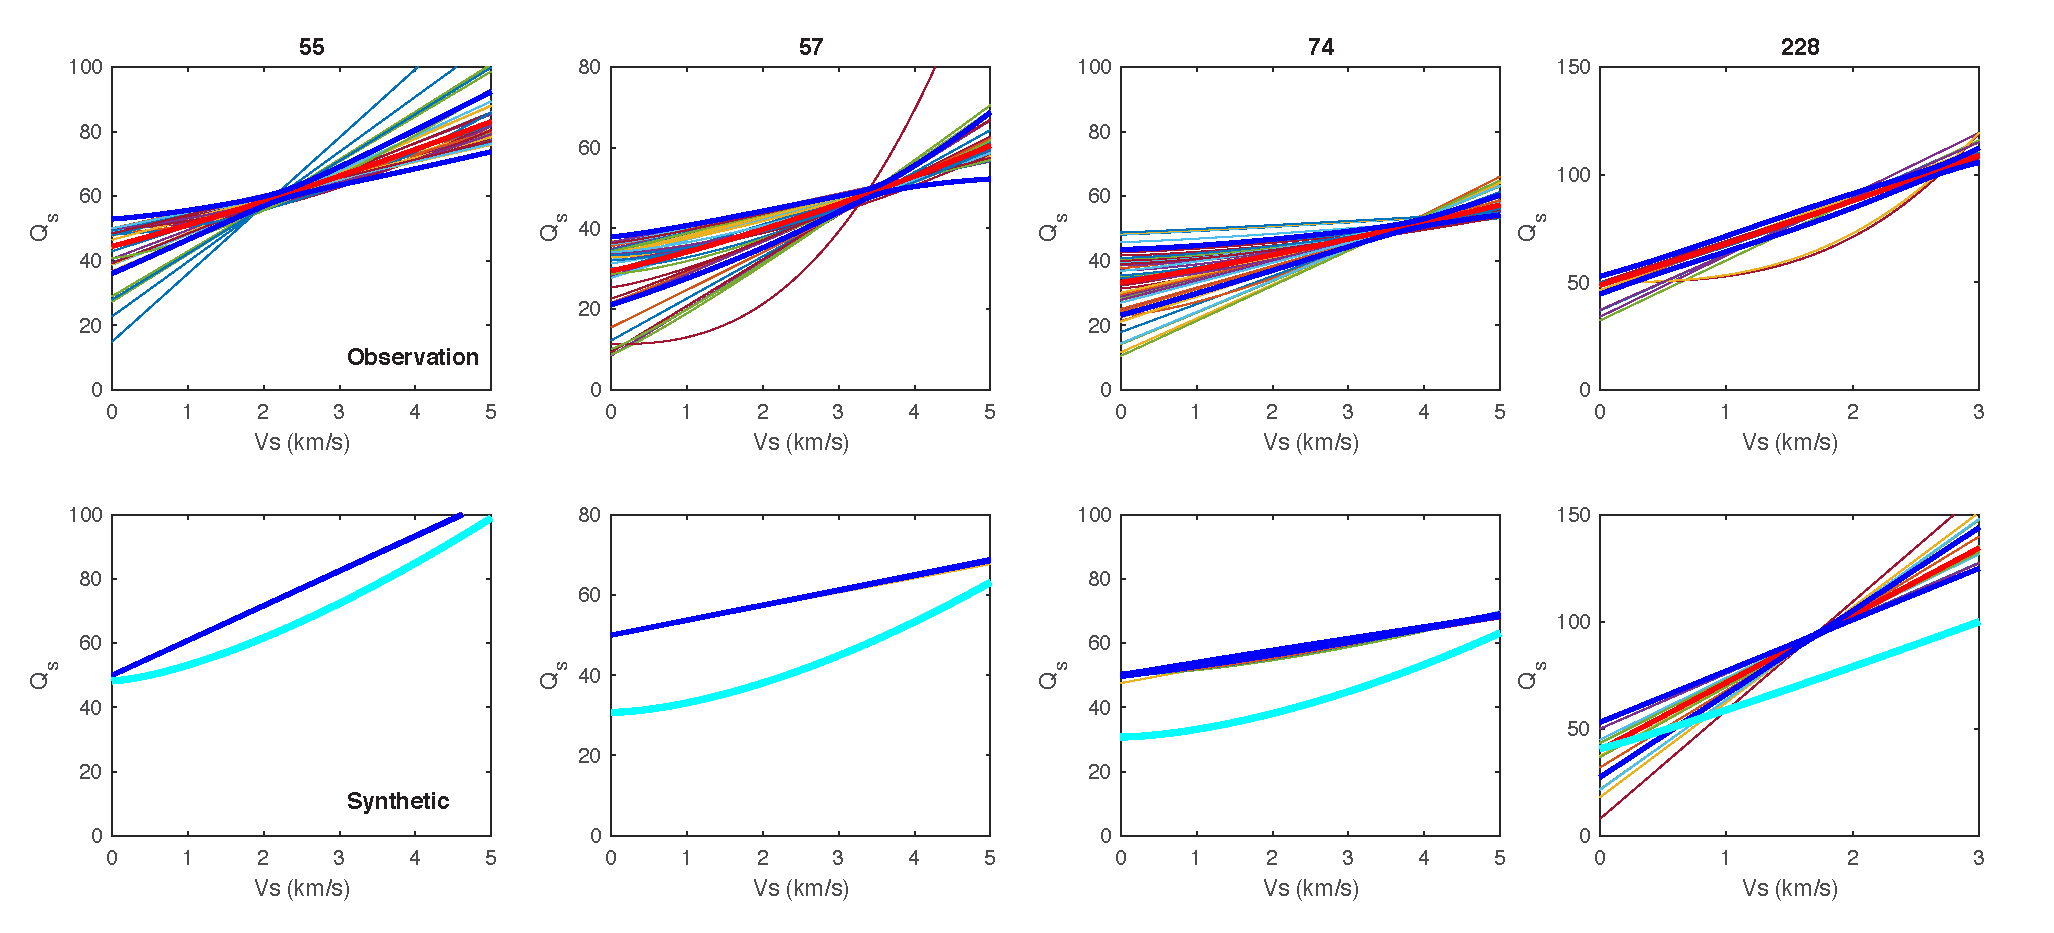
\includegraphics[width=\textwidth]{figures/pdf/unused_stations_example.pdf}
    \caption{Some of stations in the heterogeneous domain that fails the criteria. }
    \label{fig:unused_stations_example}
\end{figure}

Stations that are represented in Figure.~\ref{fig:unused_stations_example} are not used at the final process. As one can see the optimization algorithm provides very converged results at least for three of these stations. However, non of these results are according to the input parameters for target values (Cyan line). This suggest the idea that these stations are not trustable to estimate the observation values. Without the synthetic section of the analysis one arguably can use the converged results of observation. However, we can see that the algorithm is unable to retrieve accurate values. We can argue that there should not be any problem with optkmizaiotn process, rather the signal metrics are not conclusive enough to capture the input parameters. The  results show that the proposed steps can lead to very accurate and confident parameters. 

The final dataset which we believe is the most appropriate information that we can extract from our dataset in shown in the Figure.~\ref{fig:results_conservative_with_regression} . We used opacity filter to provide an estimation about the density of points in the range. We also use jitter in plotting data to give better idea of data distribution. 

  \begin{figure}[ht]
    \centering
    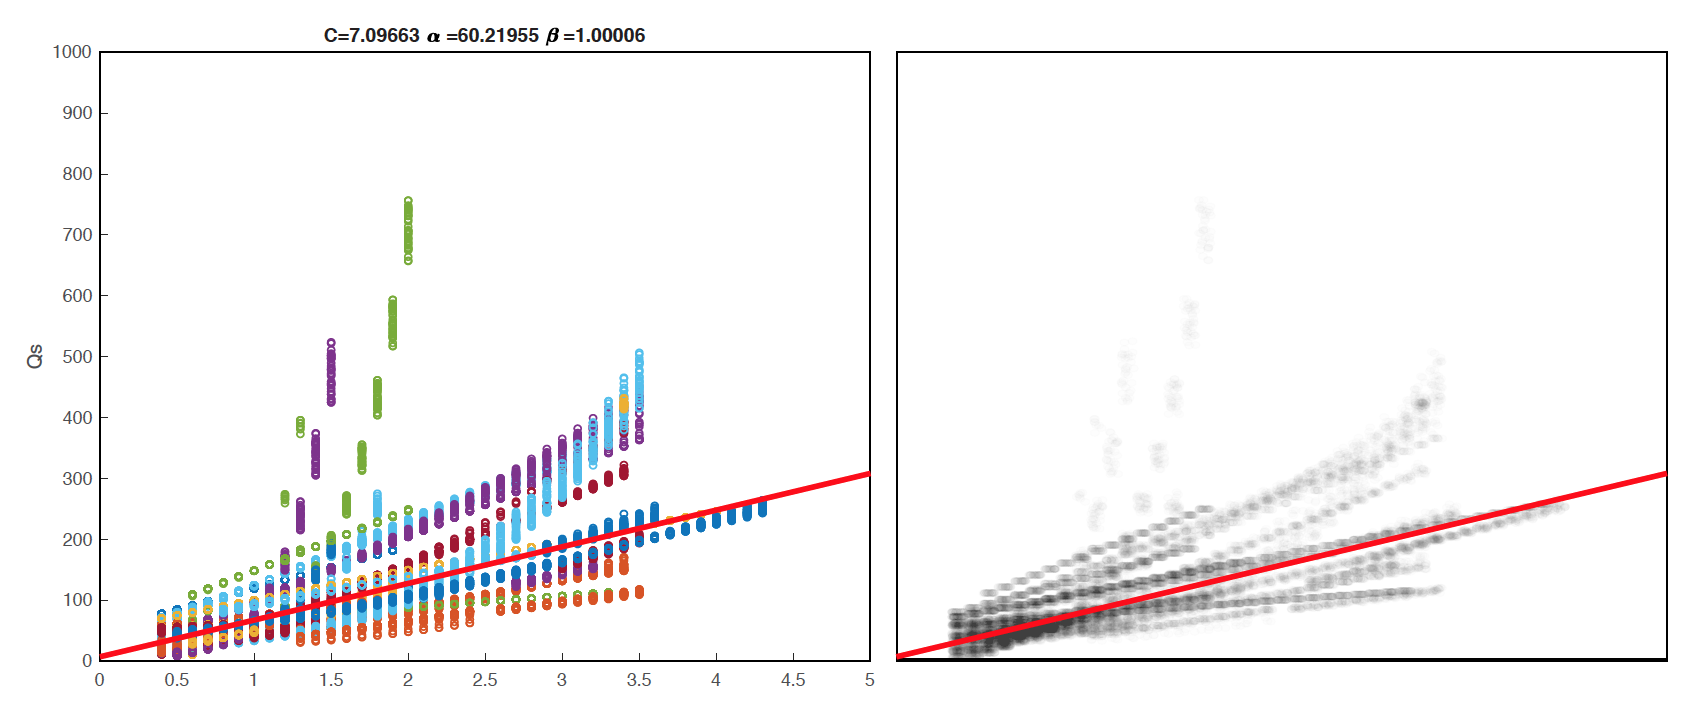
\includegraphics[width=\textwidth]{figures/pdf/results_conservative_with_regression.png}
    \caption{Scatter data of stations which passed the optimization criteria. Left: Actual data. Different colors represent different stations. Right: Same data with jitter and opacity filter to represent the data density and distribution.}
    \label{fig:results_conservative_with_regression}
\end{figure}

In computing the final equation for the Q factor, we ignore data with shear wave velocity less than 350 m/s according to minimum shear wave velocity of the simulations.  




 

